
 \chapter{Results}

Sections of this chapter, specifically the Hybrid integrated devices section,
are as a result of work which will is soon to be submitted for publication
\cite{murray2015}.

\section{Waveguide devices} \label{sec:wg_devices} As explained in the Chapter
3, by placing two waveguides in close proximity the light can couple between
each one. The power in each waveguide at a position $L$ is given by

\begin{equation} P_1(L) = I \cos^2 cL \end{equation} \begin{equation} P_2(L) = I
\sin^2 cL \end{equation}

where $I$ is the input laser intensity, $c$ is the coupling coefficient related
to the waveguide index contrast, the seperation between the guides and the
wavelength. These equations allow the design of DCs with a well defined coupling
ratio by changing the interaction length $L$. To test this a batch of chips were
fabricated with DCs of increasing interaction length $L$ and the coupling ration
was measured for each. The results are shown in Figure \ref{fig:dc_length}. The
differing black and red squares and circles are simply different chips from the
same wafer. The red line is a $\sin^2$ fit to the data. The results show good
consistency between chips, and the behaviour matches the expected sinusoid. This
allows the creation of devices with embedded DCs with any coupling ratio,
defined by the fabrication process. For example, to do on-chip Hanbury Brown and
Twiss a DC with $r = 1/2$ is needed. For a photonic quantum CNOT gate a series
of DCs with ratios $r = 1/2$ and $r = 1/3$ is needed.

\begin{figure}[h!] \begin{center}
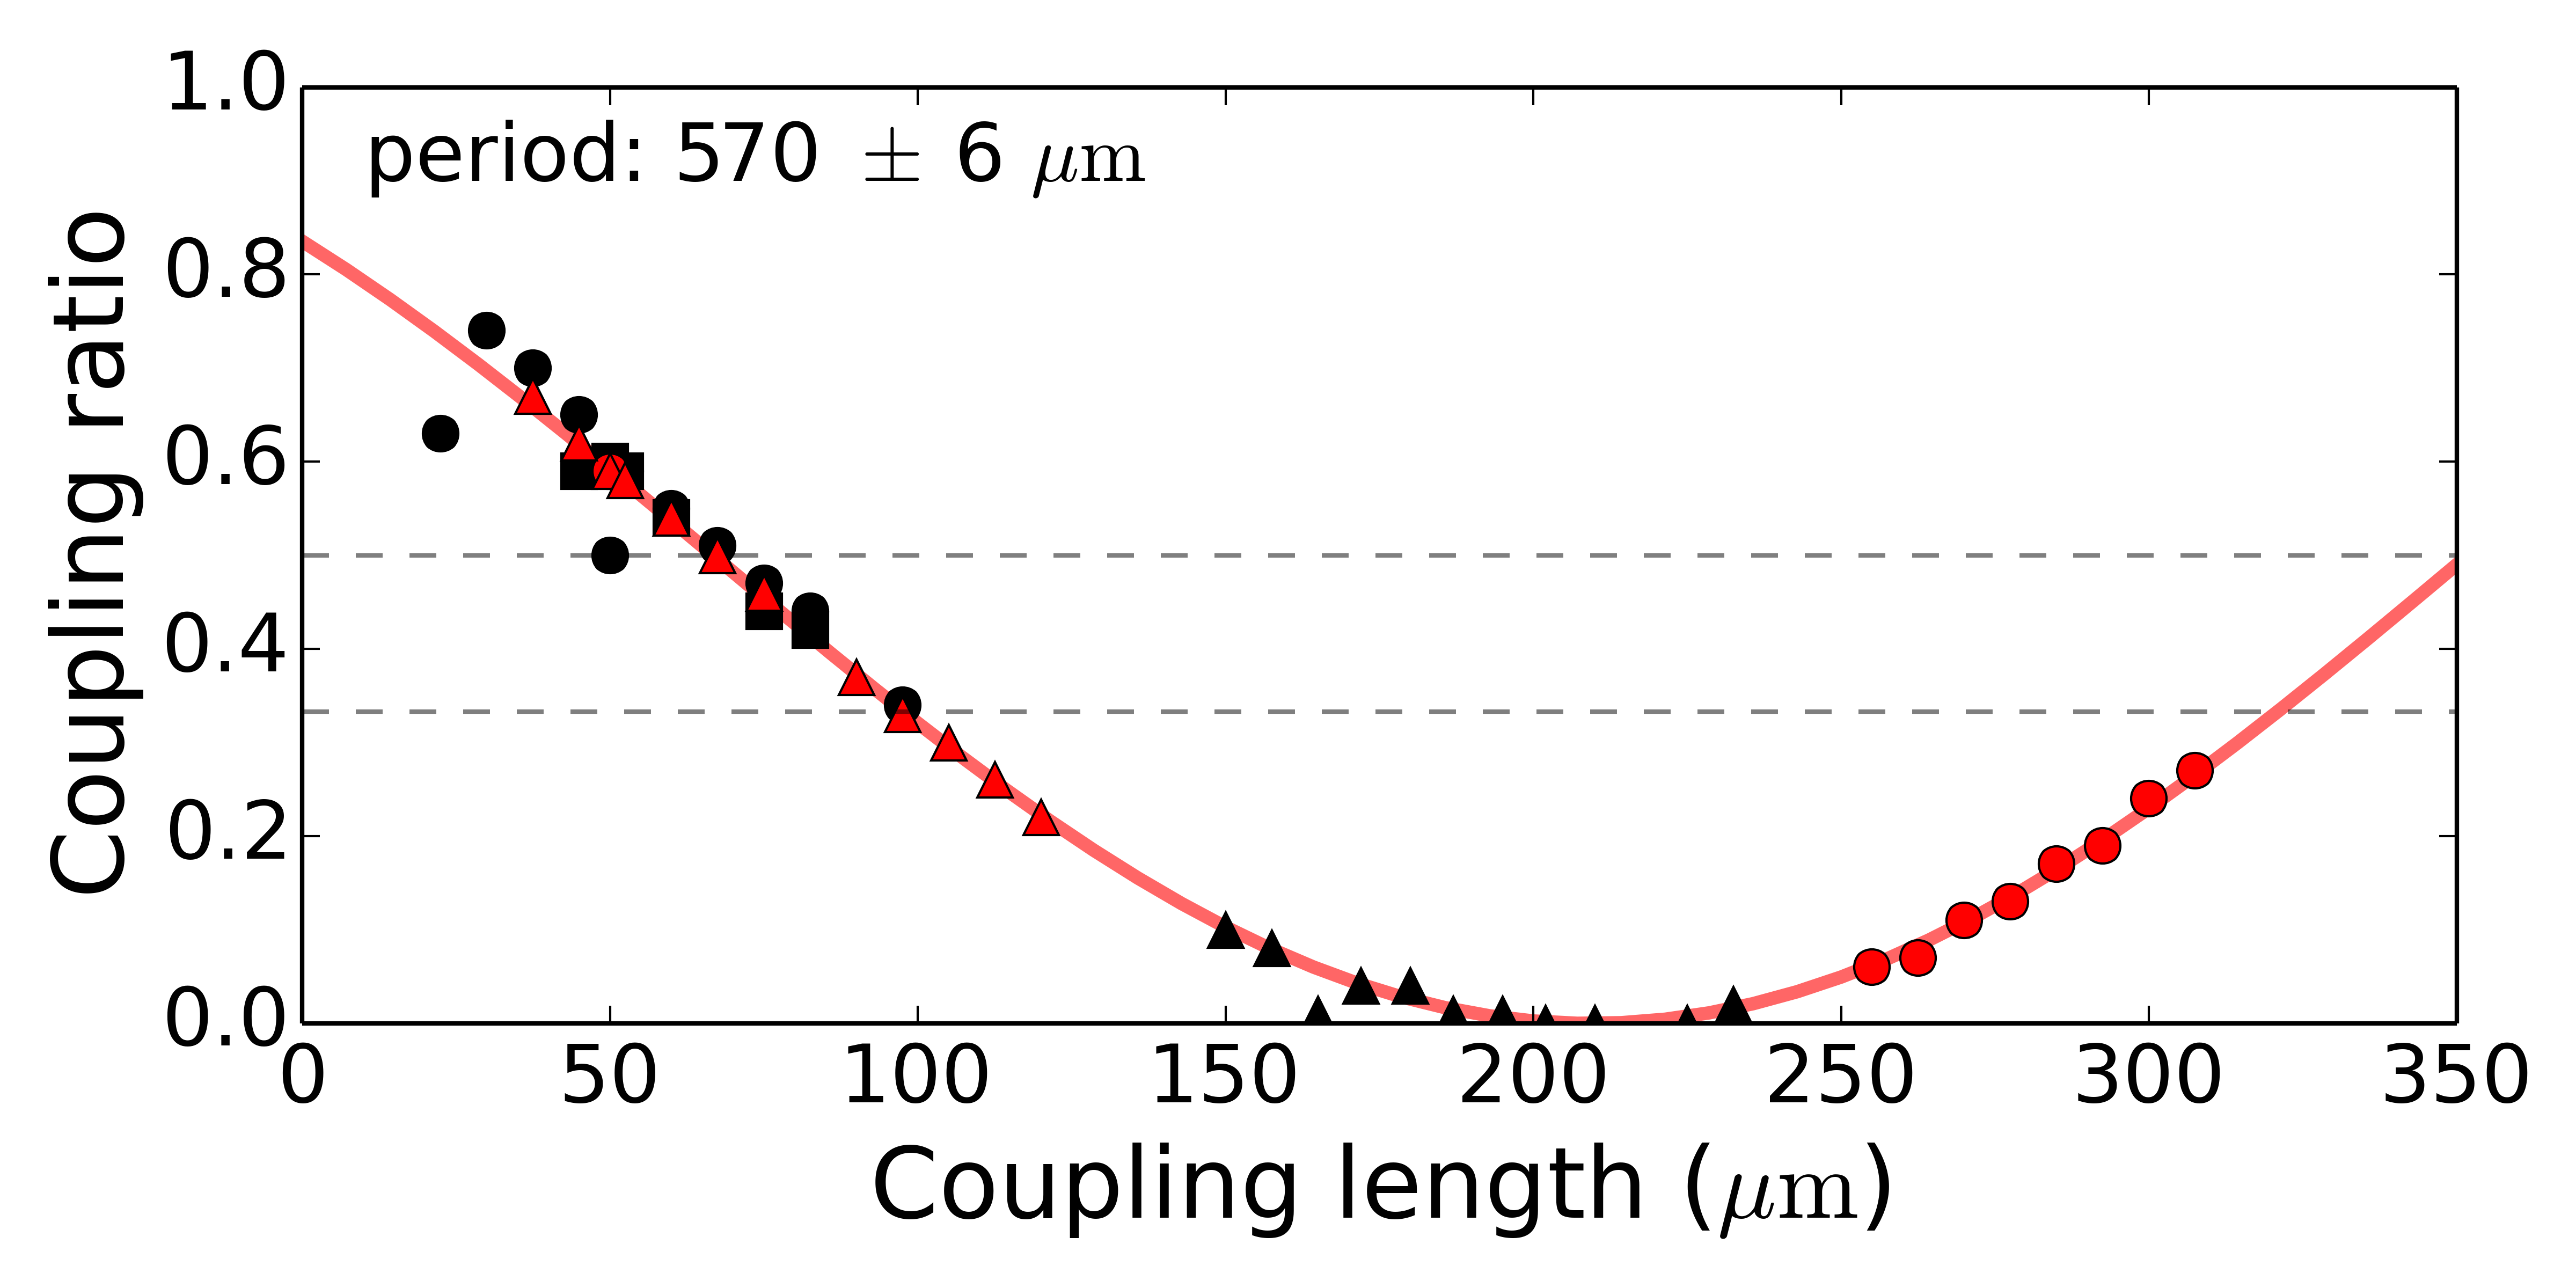
\includegraphics[width=0.7\textwidth]{images/W008_DC_processing.png}
\caption{Measured coupling ratio vs interaction length for a batch of waveguide
chips. The results show the expected smooth sinusoidal behaviour.}
\label{fig:dc_length} \end{center} \end{figure}

Another important parameter for a waveguide device is its operating wavelength,
depending on the III-V source used, the waveguide device would need to operate
in the range 900-950nm. The properties of a DC will change depending on the
wavelength of the light. To check this, one DC was analysed by varying laser
wavelength and monitoring the coupling ratio, this result is shown in Figure
\ref{fig:dc_wv}.

\begin{figure}[h!] \begin{center}
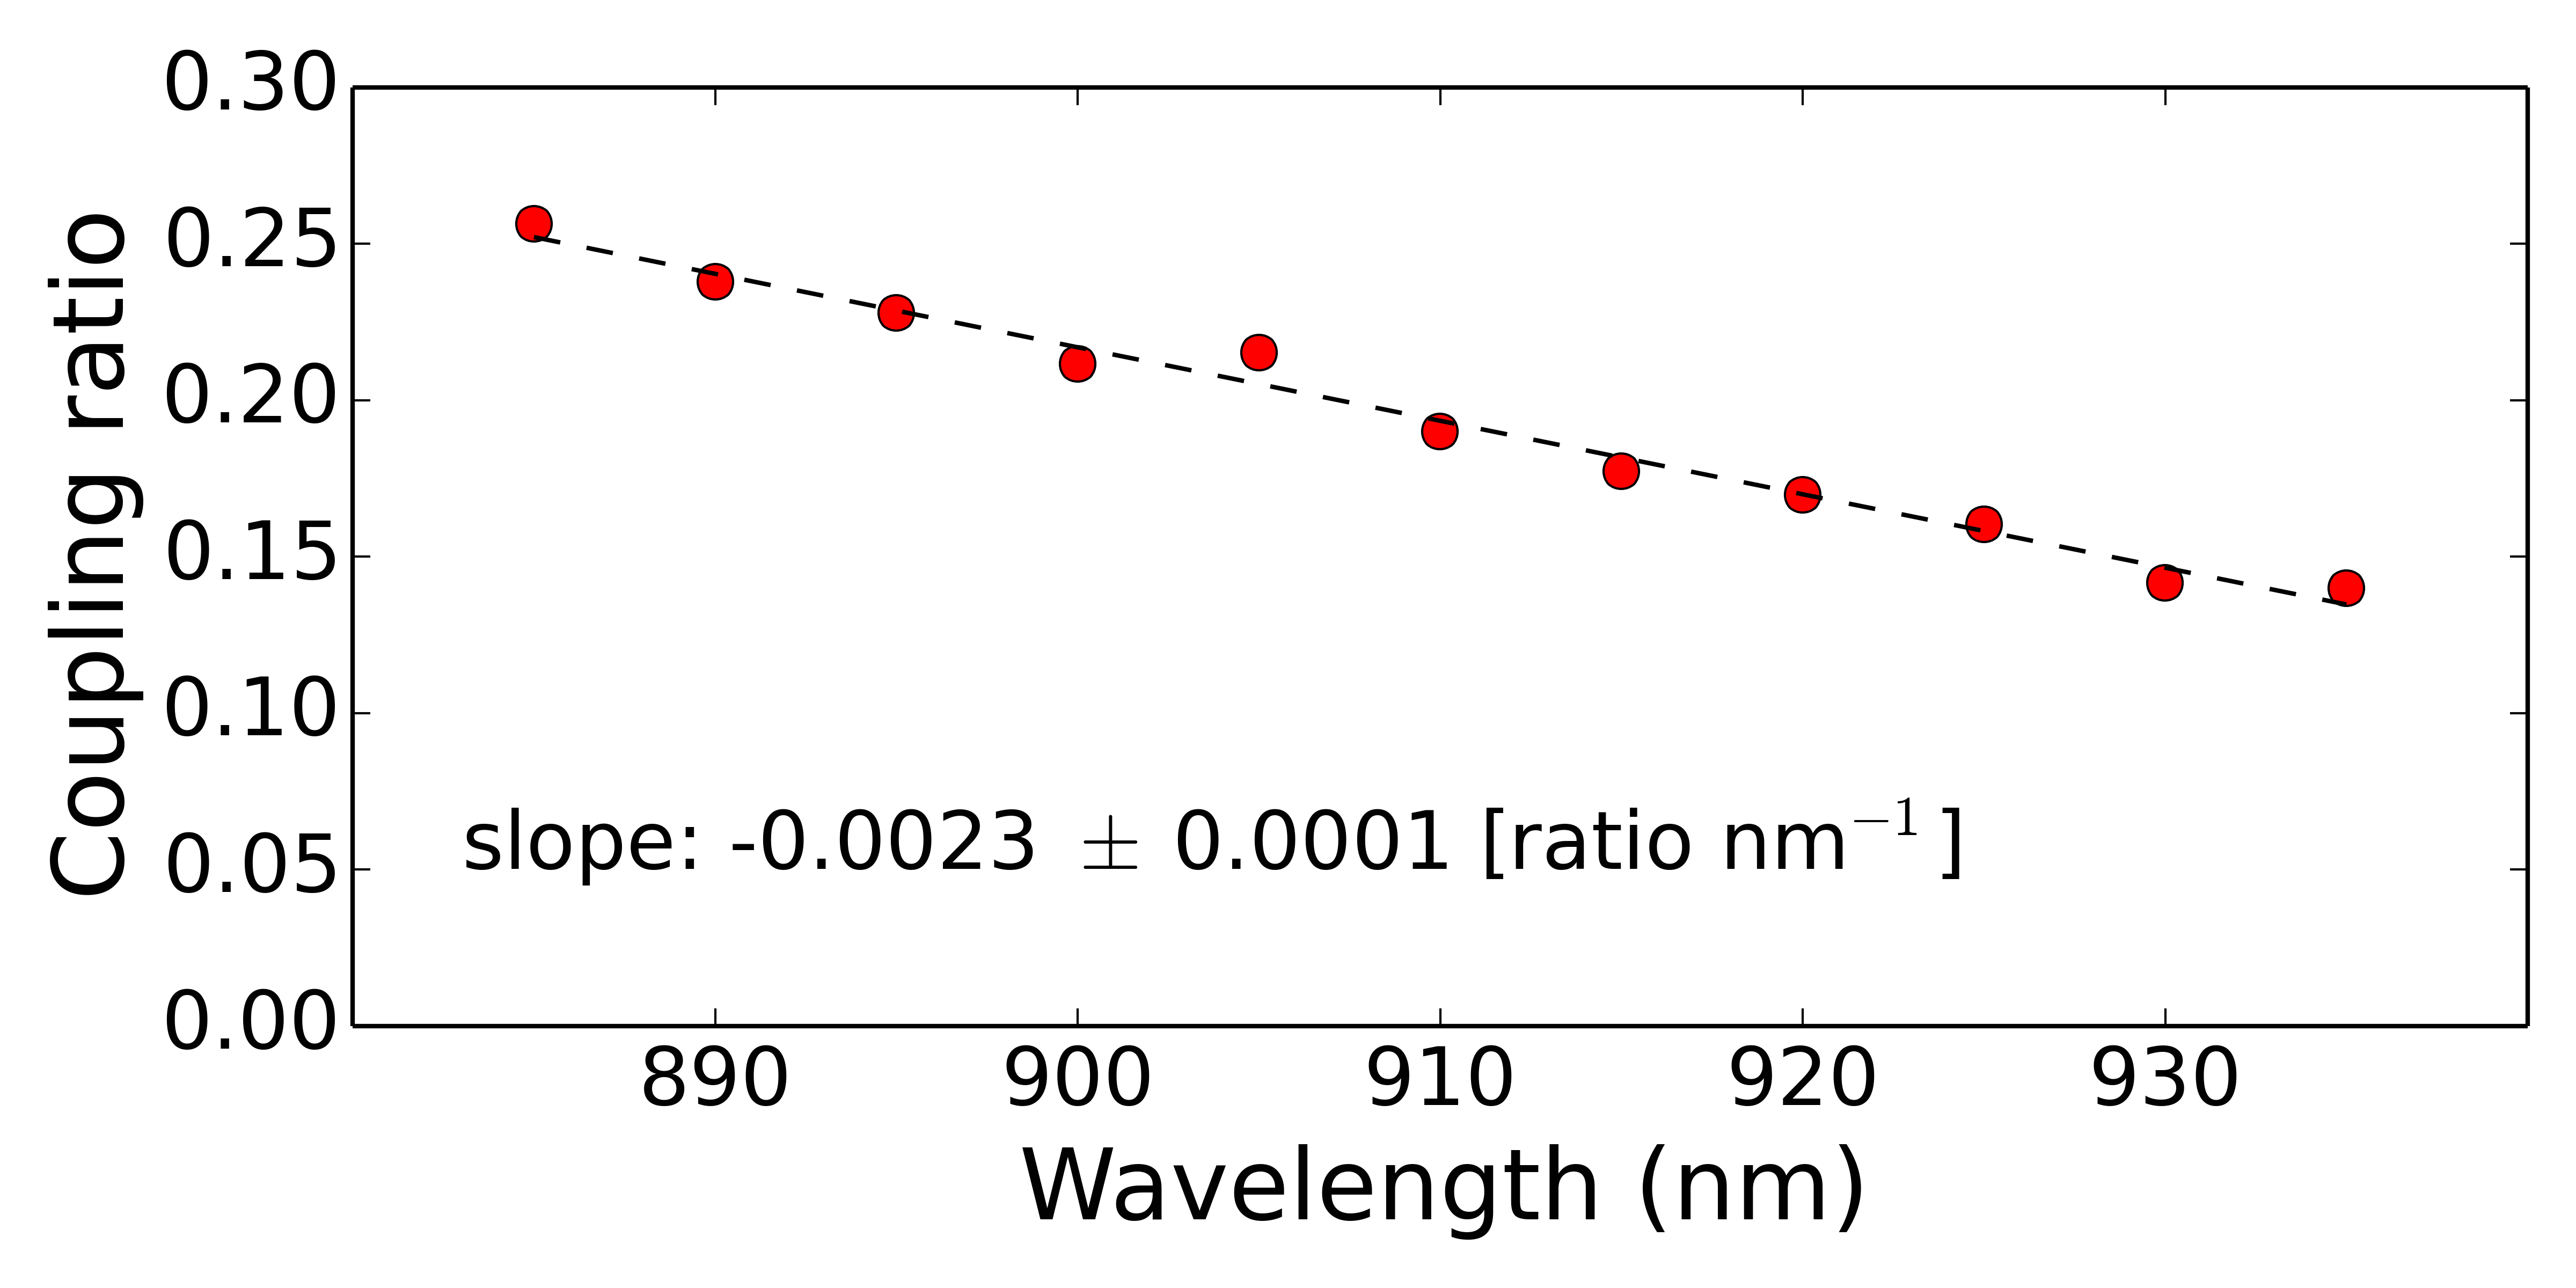
\includegraphics[width=0.7\textwidth]{images/W009C01_DV_WV_processing.png}
\caption{Measured DC coupling ration vs laser wavelength for a device. The red
line is a linear fit to the data.} \label{fig:dc_wv} \end{center} \end{figure}

As is seen in the figure, there is a linear decrease in the coupling ratio with
increasing wavelength for the measured chip. In general the wavelength
dependence is always linear, however whether the slope is positive or negative
depends on othe chip parameters, such as length, period of the length dependance
and index contrast.

\begin{figure}[h!] \begin{center}
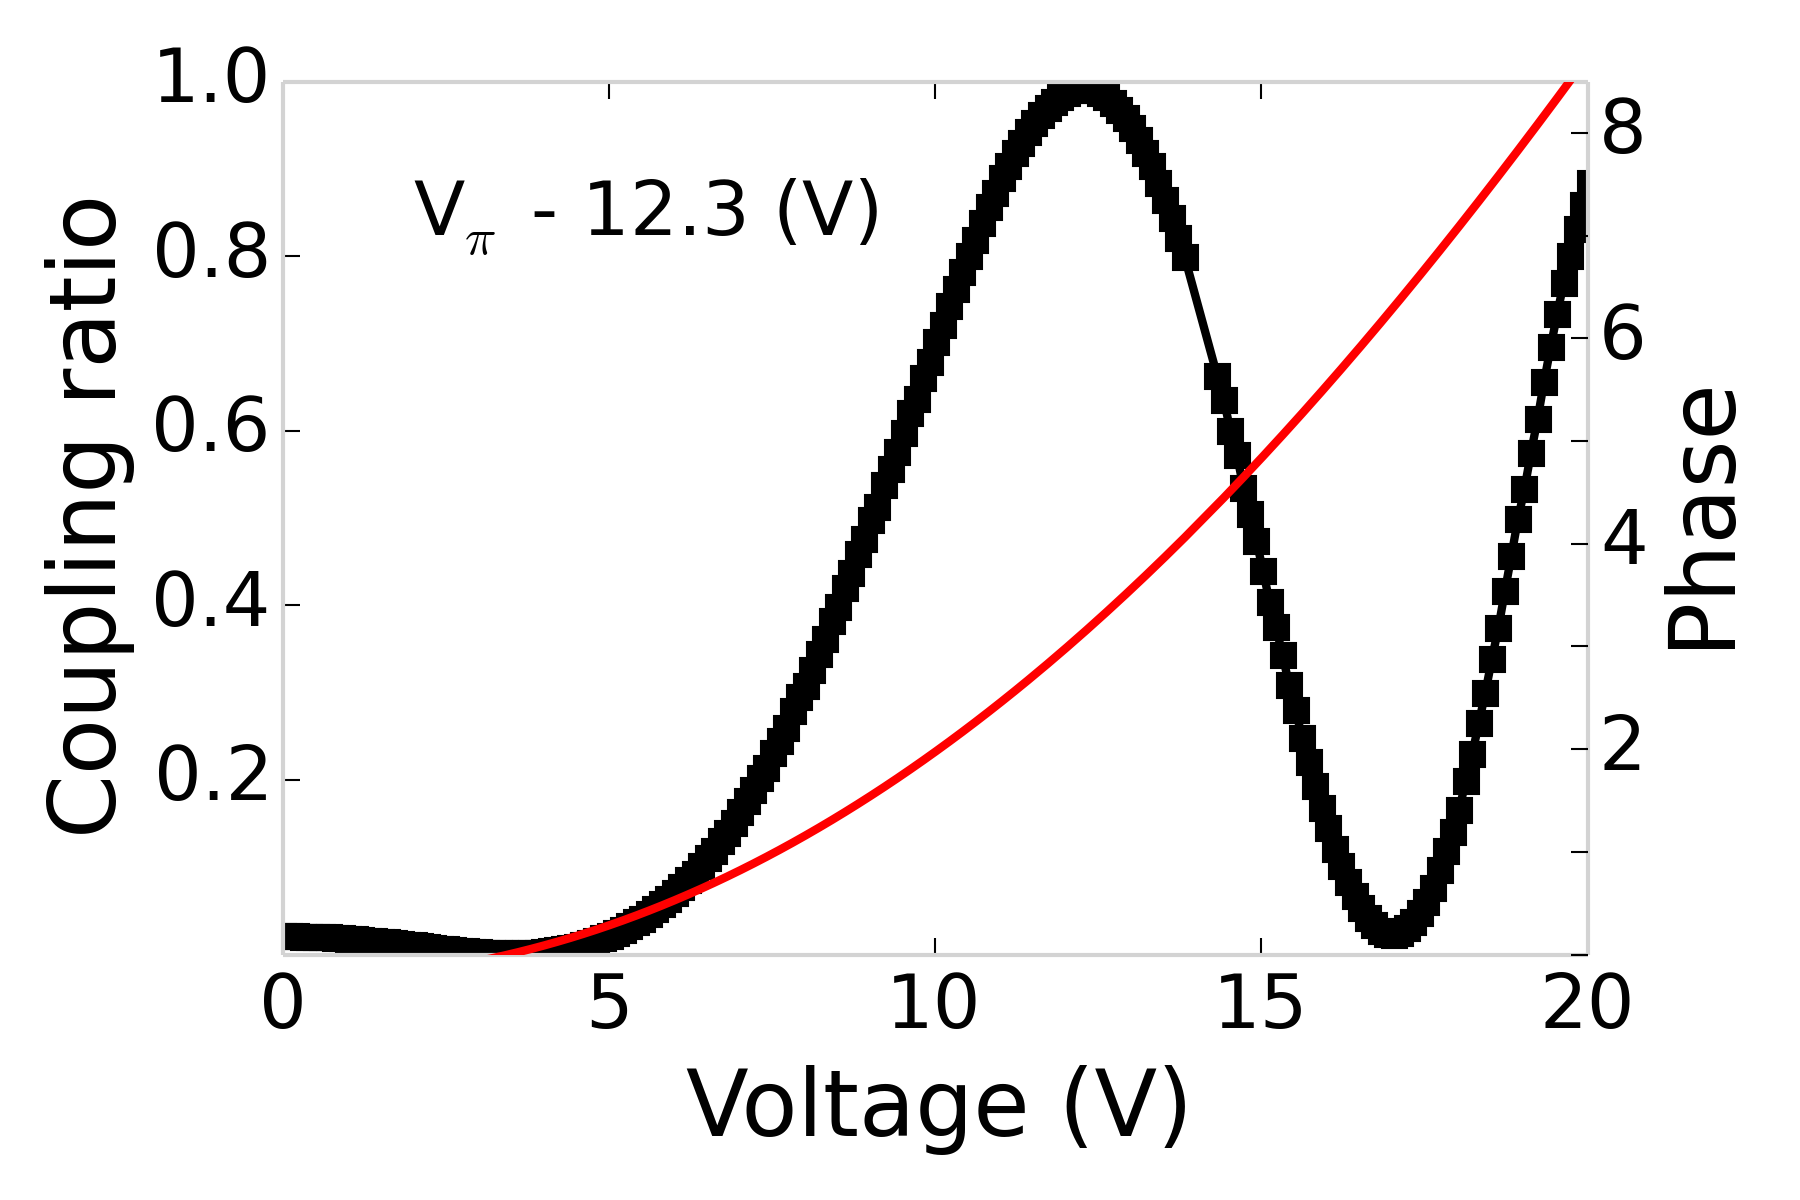
\includegraphics[width=0.7\textwidth]{images/W010_C06_phase_voltage_MZ1_5_5_6.png}
\caption{Performance of an SiON based Mach Zehnder interferometer. The black
line traces the coupling ratio vs applied voltage and the red line is the phase
calculated from the data.} \label{fig:mz} \end{center} \end{figure}

Mach Zehnder interferometers are very interesting devices for their applications
in quantum computing, by way of a qubit preparation device, and in
telecommunications, as a light modulator. The MZs were fabricated as described
in Chapter 2. The coupling ratio was monitored as the heater voltage was varied.
The result is shown in Figure \ref{fig:mz}. The black squares are the coupling
ratio as the voltage was varied and the red line is the calculated phase. The
phase was calculated using a pre-established model
\cite{matthews2009manipulation}. The visibility of this MZ was 99.7 $\pm$ 0.06 \%.
To apply a $\pi$ phase shift to the light in one arm in this case would need
12.3 V applied to the heater.

\section{Hybrid integrated devices}

Various approaches for embedding QDs into integrated circuits are being
explored. Photonic crystal waveguides yield high coupling efficiency of the QD
emission into the in-plane propagating waveguide mode \cite{schwagmann2011chip}.
They have also demonstrated in-plane indistinguishable photons
\cite{kalliakos2014plane}. QDs integrated with ridge waveguides in GaAs have
been reported integrated with on-chip superconducting single photon detectors
\cite{reithmaier2013chip}. Air clad GaAs ridge waveguides have also demonstrated
QD integrated directional couplers \cite{prtljaga2014, jons2014monolithic}.
Other approaches use heralded single photons from spontaneous parametric down
conversion integrated with waveguide chips \cite{meany2014hybrid} however this
approach lacks the deterministic emission of quantum dots.

In this section the results from an integrated platform for hybrid integration
of III-V QDs into silicon oxynitride waveguides are presented. A GaAs chip
containing InAs quantum dots are bonded orthogonally to the SiON chip such that
the photons emitted from the surface of the GaAs chip are routed into a guided
mode. The quantum dots are embedded in a low quality factor distributed Bragg
reflector cavity with alternating layers of AlAs and GaAs. The SiON chip
consists of a waveguide to deliver laser excitation light to the quantum dots
and a return line consisting of a MZ interferometer. The MZ can act as a qubit
preparation device for the single photons emitted from the QD. If a single
photon impinges on a 50:50 MZ then the single photon will be placed into a path
encoded superposition of each output mode. The probability amplitude of being in
each mode can be tuned by the active modulation of the MZ. The hybrid method of
coupling was modelled by finite difference time domain simulations to calculate
the mode overlap of the quantum dot source and the propagation mode of the
waveguide; this also allows a calculation of the efficiency. The interferometer
tuning is based on local heating of one arm. At zero tuning the light is split
and the two output waveguides are bonded to a V-groove array of fibres. This MZ
beam splitter allows on chip Hanbury Brown and Twiss correlations to verify the
single photon nature of the light source. The MZ can be tuned to modulate the
light, allowing routing of the light into either or both output arms.

\subsection{Simulations and design}

\begin{figure}[h!] \begin{center}
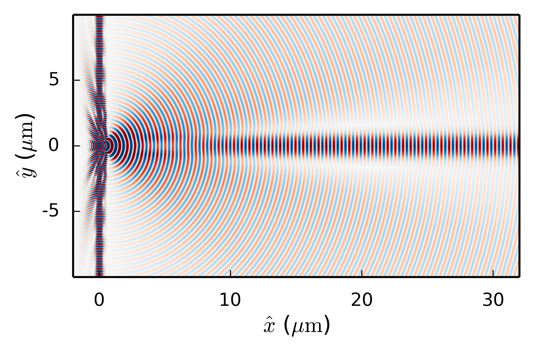
\includegraphics[width=0.8\textwidth]{images/sim.png} \caption{Finite difference
time domain simulation of a QD dipole emitting in a cavity and the emission
being guided by the SiON core.} \label{fig:sim} \end{center} \end{figure}

As described in Chapter 2 the characteristics of the device were simulated by
using the finite difference time domain package MEEP \cite{oskooi2010meep,
mandelshtam1997harmonic}. A $\hat{z}$ oriented dipole emitter was placed in the
centre of the cavity spacer aligned to the centre of the waveguide. A perfectly
matched layer was placed at the edges of the simulation domain to absorb all
light and prevent unwanted reflections. The $\hat{z}$ component of the electric
field is shown in Figure \ref{fig:sim}. There is a clear emission pattern along
the waveguide core. The efficiency of this device was also determined
theoretically. A bounding box which records the Fourier transformed fields was
placed at the edge of the domain and just inside the perfectly matched layer.

From this bounding box the total power spectrum is recorded when the system is
excited with a short Gaussian pulse. Another flux plane is placed across the
waveguide. The waveguide core size was 1.6 $\mu \mathrm{m}$ and the far field
propagating mode has a spatial $1/e$ width of 1.88 $\mu \mathrm{m}$ which was
chosen as the size of the waveguide flux plane. It is placed sufficiently far
from the surface of the III-V so that only the waveguide propagating mode is
measured. Taking the ratio of the light propagating in the waveguide to the
total in the bounding box gives the efficiency of the hybrid collection system.
At the centre of the cavity wavelength the efficiency is 2.8\%. For a QD
emitting into free space with no cavity a collection of 0.5\% can be expected
into a 0.5 NA objective. When the QD is in a cavity the efficiency can rise to
7\% depending on the number of mirror repeats and the numerical aperature of the
collection objective. For the device presented here the numerical aperature of
the waveguide is 0.35 and the III-V sample has a distributed bragg reflector
cavity with 12 repeats below the QD layer and 2 repeats above. This efficiency
of 2.8\% is almost exactly in line with what has previously been estimated for
free space collection with the same NA and same number of repeats
\cite{bennett2006single}.

\subsection{Measured results}

\subsubsection{Hybrid integration}

\begin{figure}[h!] \begin{center}
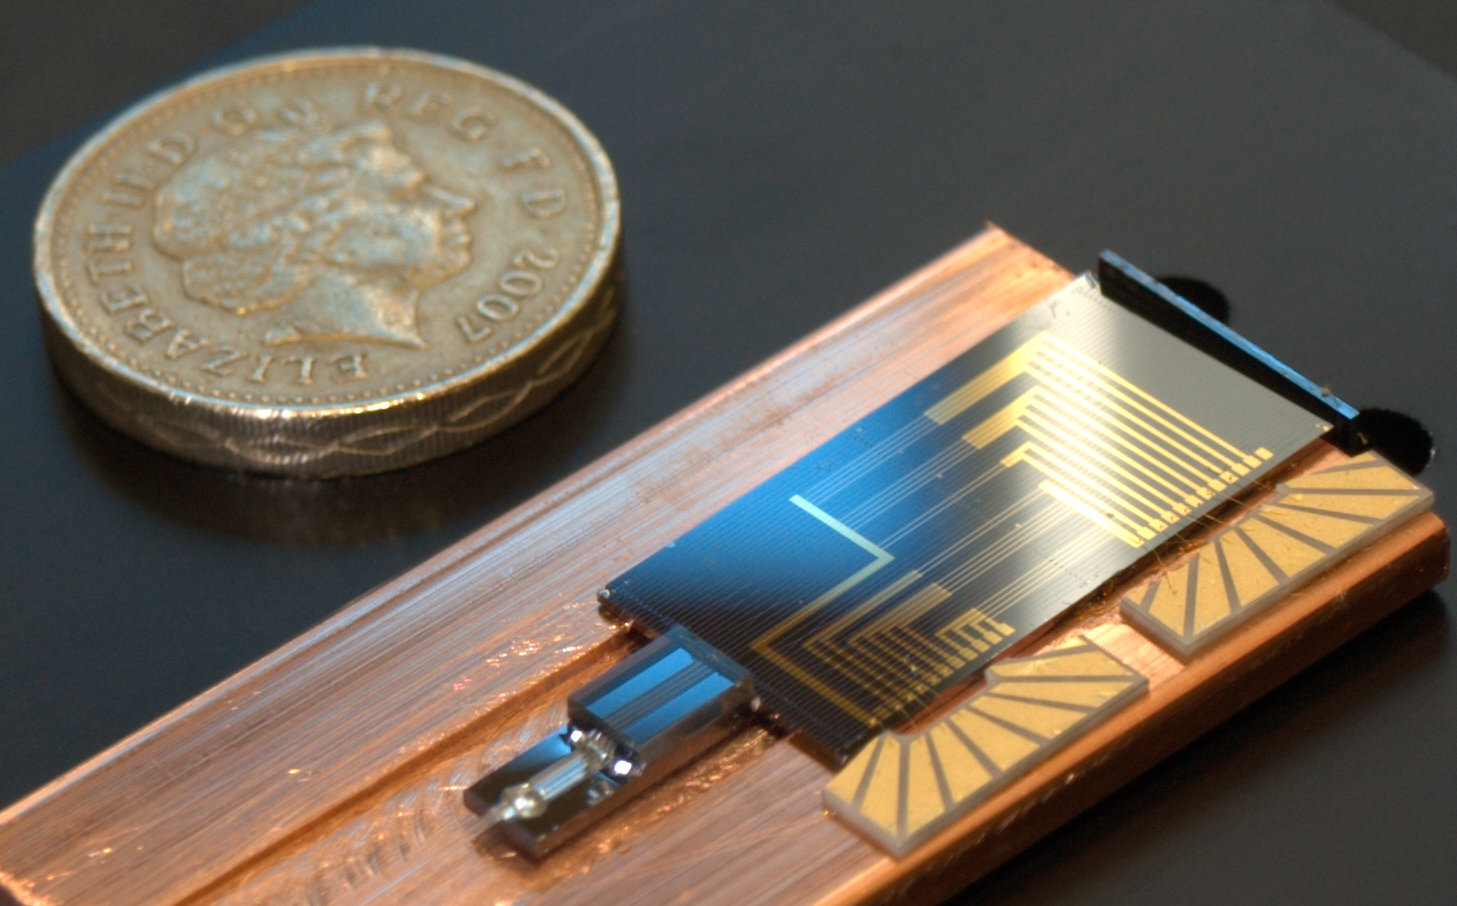
\includegraphics[width=0.7\textwidth]{images/h2.jpg} \caption{Photograph of an
example bonded device.} \label{fig:photo} \end{center} \end{figure}

Figure \ref{fig:photo} shows a photograph of an example device. A strip of
microcavity wafer containing QDs is bonded to one end of the SiON waveguide
chip. The orthogonal bonding method allows the surface emission from the QD to
be collected by the waveguide. This orthogonal bonding is a major advantage of
this hybrid integration method. The surface emission from the QD can be easily
optimised by growing a distributed Bragg reflector cavity and/or creating a
micropillar structure. Previous reports show efficiencies of out of plane QD
collection as high as 0.75 into free space high numerical aperature objectives
\cite{claudon2010highly, munsch2013dielectric}. In SiON the waveguide numerical
aperature is limited by $\sqrt{n_{core}^2 - n_{clad}^2}$, where $n_{core} =
\mathrm{1.55}$ and $n_{clad} = \mathrm{1.51}$. The hyrid platform also has the
potential for diode structures to be created for electrically driven or tuneable
QD devices integrated with the waveguides. High coupling efficiencies have been
reported for some in-plane integration techniques like photonic crystal
waveguides\cite{schwagmann2011chip, arcari2014near}, however as of yet no
directional couplers or active modulation have been demonstrated. In the device
presented here the photons are routed into the waveguides, two sequential
directional couplers form a MZ with a nichrome heater applying a local phase
shift to one MZ arm. This SiON technology is compatible with the creation of
arbitrary designs of beamsplitters, MZs and phase shifters. As explained in the
previous chapter, a polarisation maintaining V-groove array is aligned and
attached to the waveguides for collection and the device is cooled to 4K for the
duration of the experiment.

\begin{figure}[h!] \begin{center}
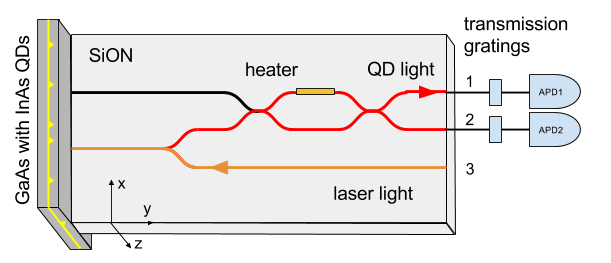
\includegraphics[width=0.8\textwidth]{images/hyb.png} \caption{Schematic of the
experiment.} \label{fig:schem} \end{center} \end{figure}

Figure \ref{fig:schem} shows the optical schematic of the experiments. A single
channel delivers laser light. The QD light is returned through the MZ and
collected into fibre by the V-groove array. The V-groove fibres are sent
directly to a spectrometer. For time resolved experiments transmission gratings
are used to spectrally filter the emission before sending the light to avalanche
photodiodes.

\begin{figure}[h!] \begin{center}
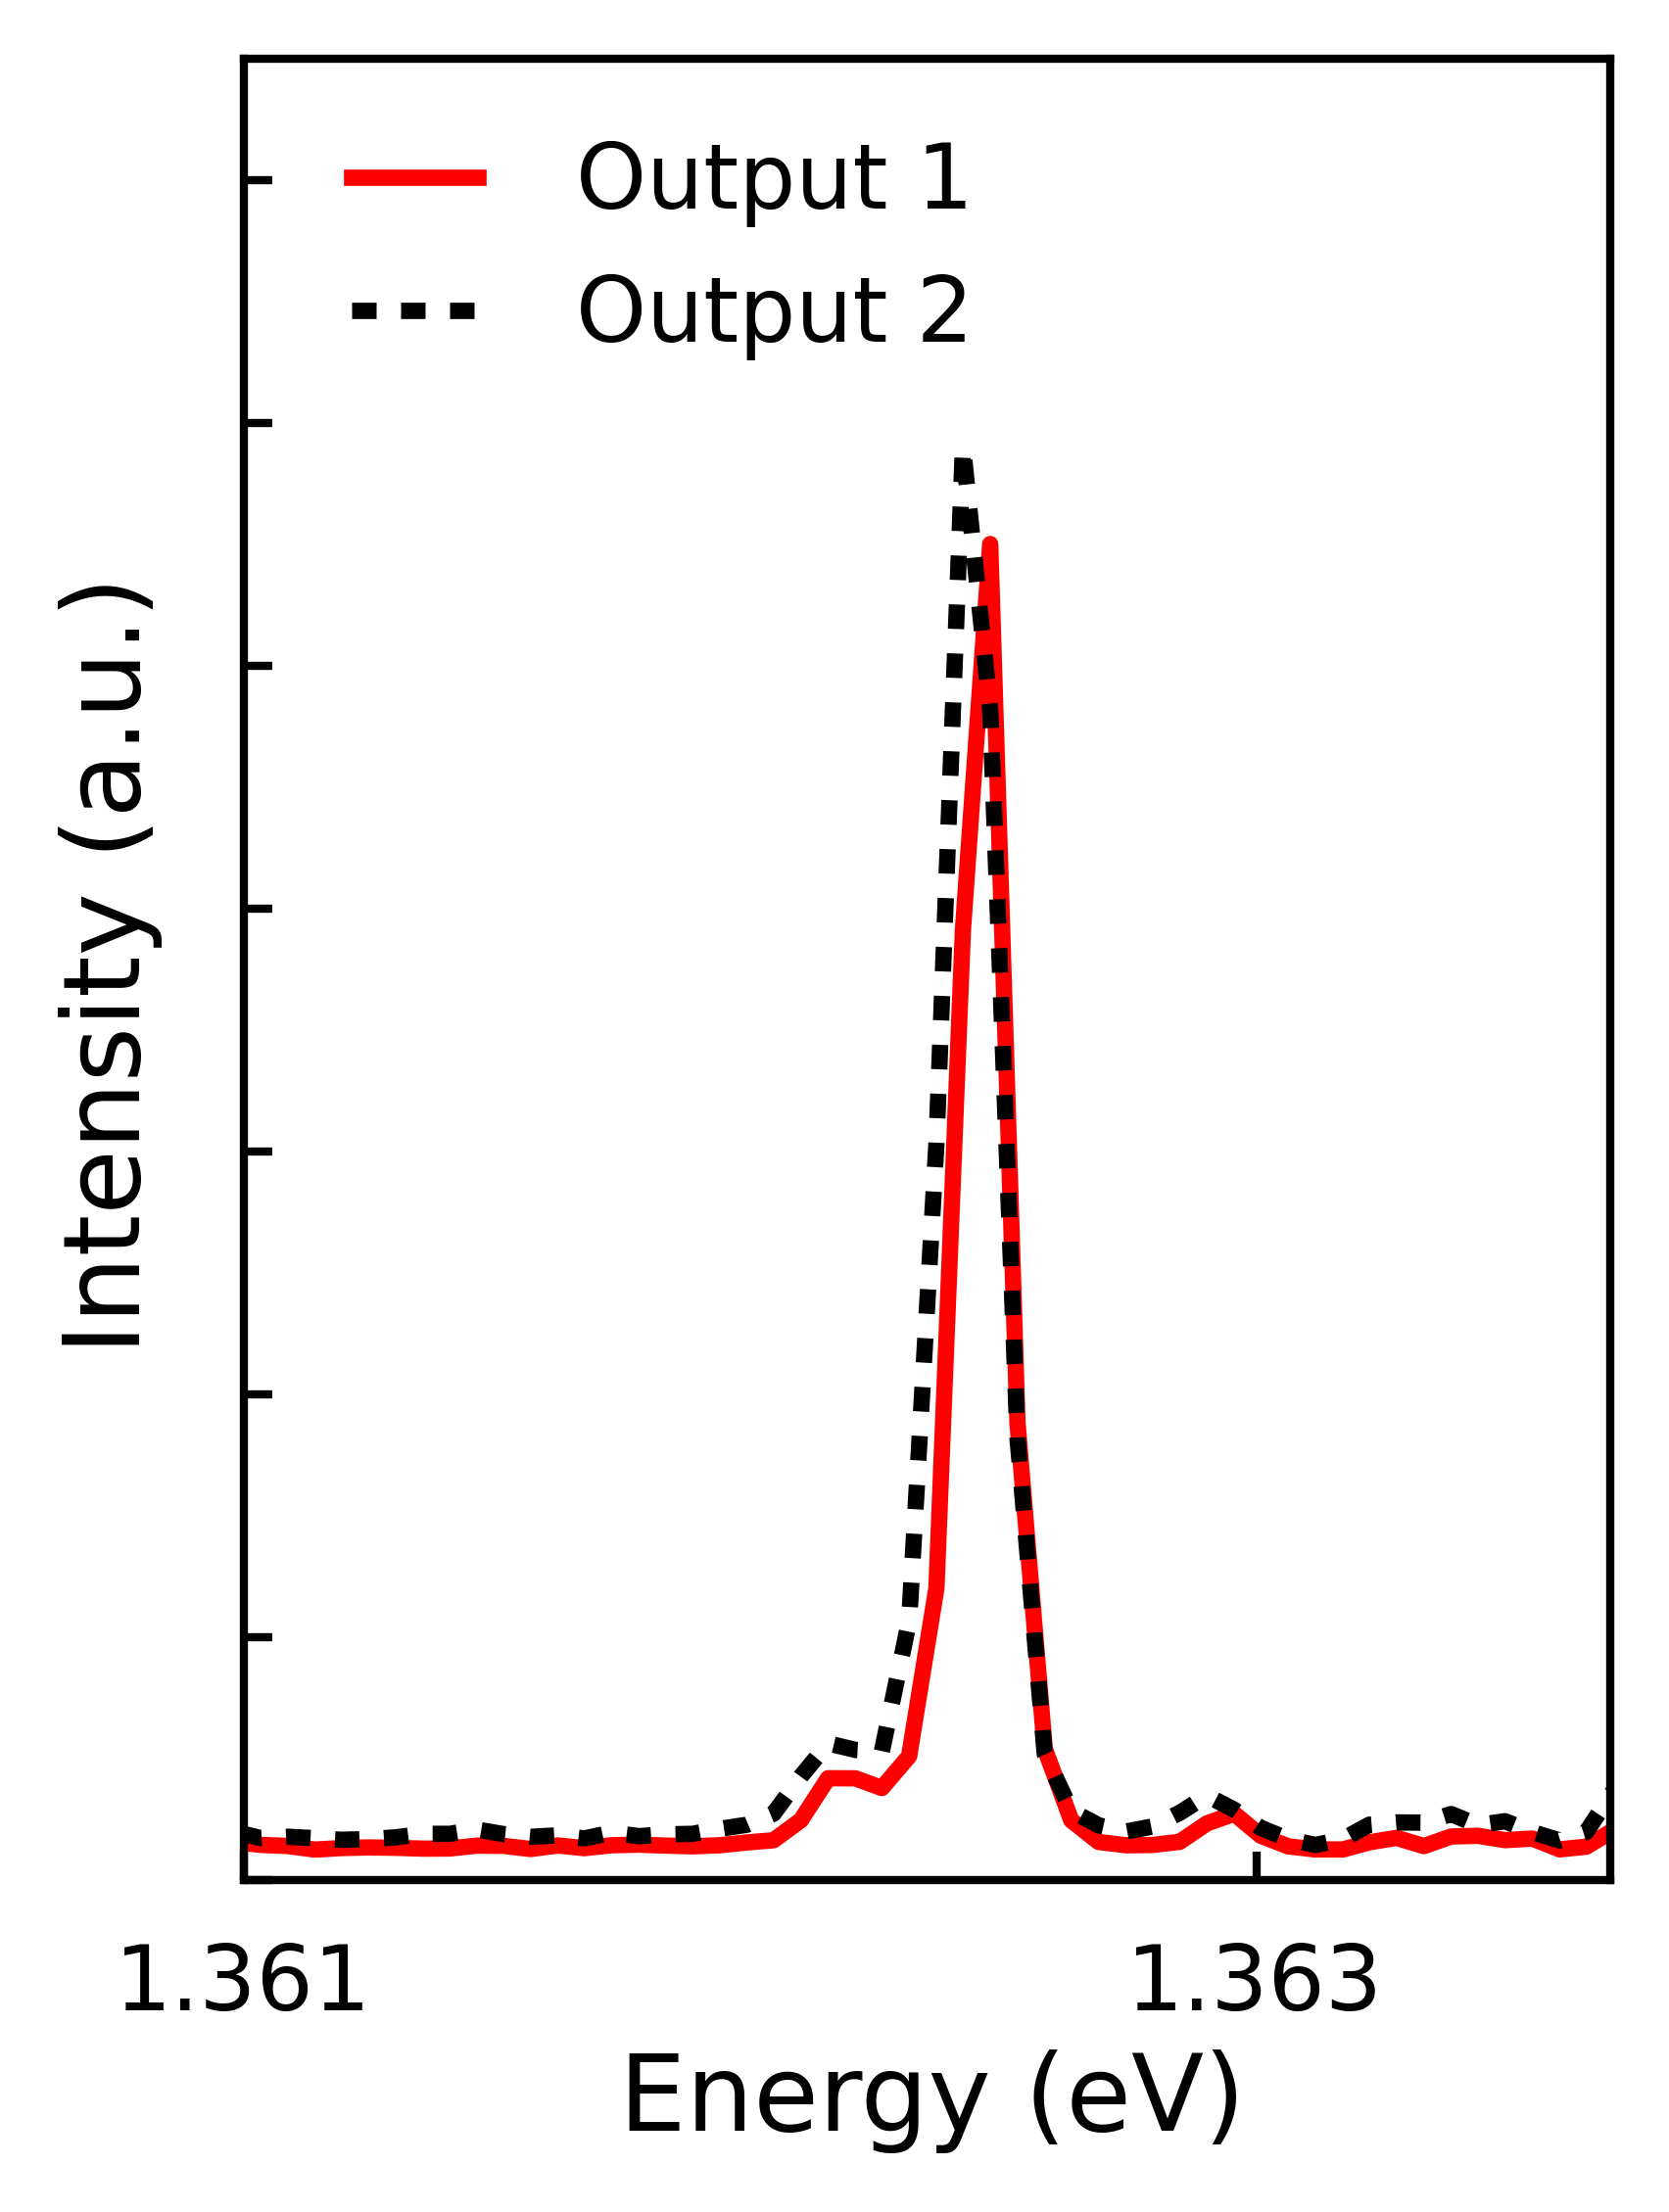
\includegraphics[width=0.45\textwidth]{images/spec.png} \caption{Spectrum of a
quantum dot from both output ports.} \label{fig:spec} \end{center} \end{figure}

The integrated device is fixed and there is no freedom to analyse different QDs
on the III-V sample once the bonding is complete. This creates stability and no
drifting in emission intensity is seen over the course of 12 hours. The QD
intensity as a function of time is plotted in Figure \ref{fig:stab}. A
reasonably high density QD sample is used to ensure that a dot which is emits in
the centre cavity mode is aligned with a waveguide. The QD layer was made of
InAs inside a $2\lambda$ spacer. The central cavity wavelength is at 910nm. The
spectrum from both outputs of the device can be seen in Figure \ref{fig:spec}.
The MZ was tuned to 50:50, and it is seen that the spectrum from both output
arms is identical. The QD analysed was the one at the centre of the cavity mode
at 1.362 eV.

\begin{figure}[h!] \begin{center}
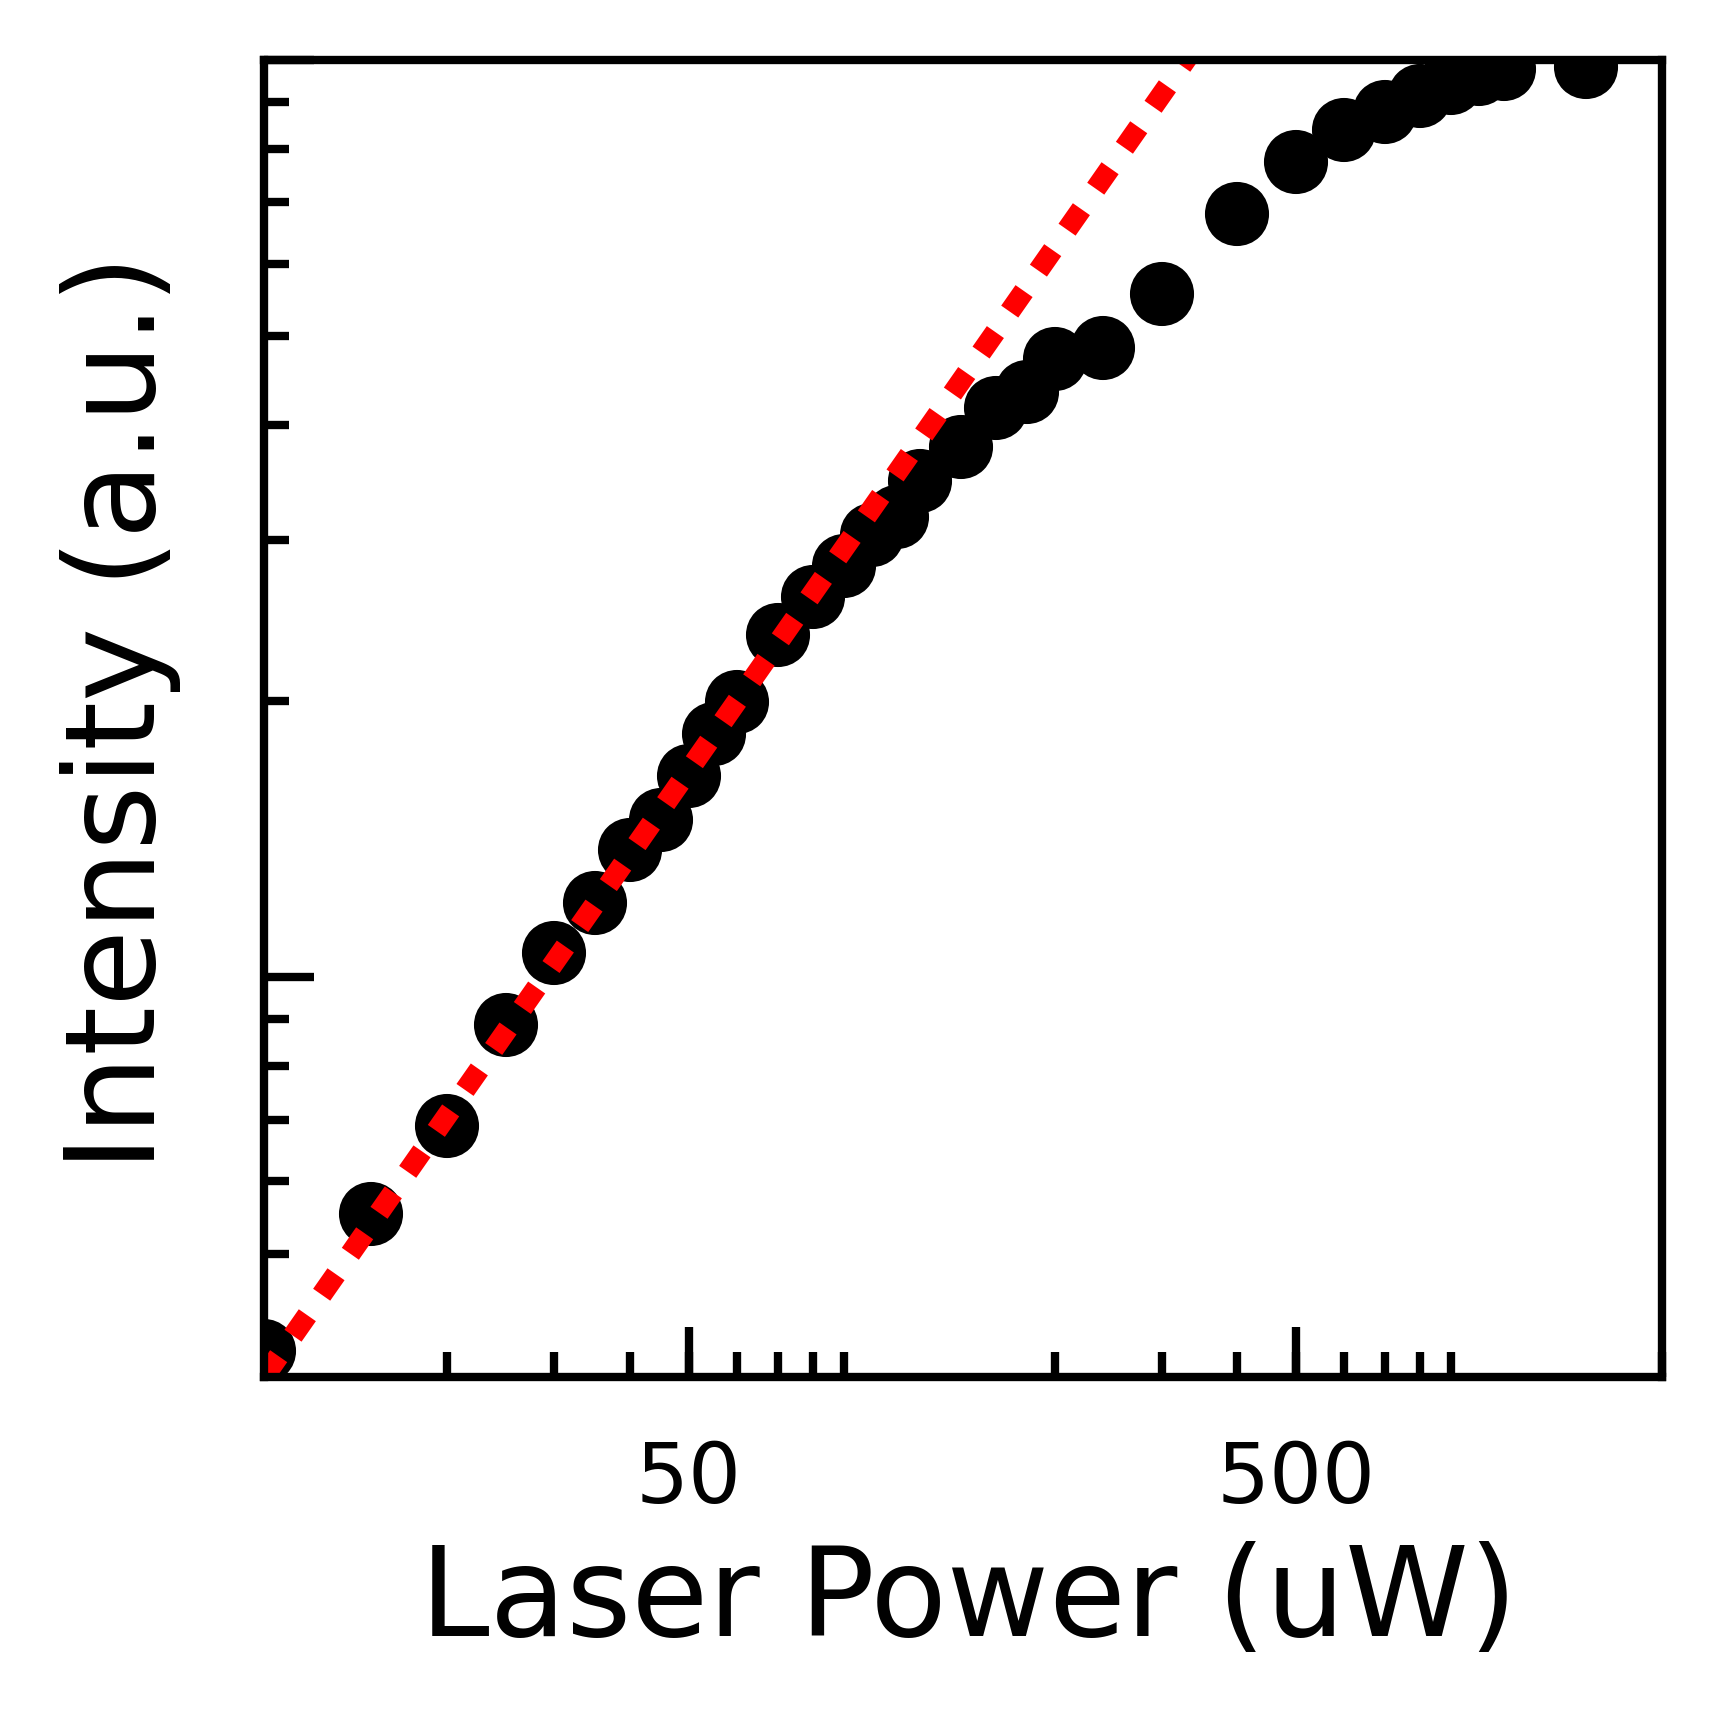
\includegraphics[width=0.45\textwidth]{images/pdep.png} \caption{Recorded
dependance of the QD emission intensity on the laser power, the solid line is a
linear fit to the data.} \label{fig:pdep} \end{center} \end{figure}

A power dependence was recorded, seen in Figure \ref{fig:pdep}. The emission,
before saturation, is approximately linear (P$^{0.95}$) implying an exciton and
not a higher order complex \cite{grundmann1997theory}. The peak exhibits no fine
structure splitting typically seen in a neutral exciton
\cite{bayer2002fine,gammon1996fine} so it is likely charged.

\begin{figure}[h!] \begin{center}
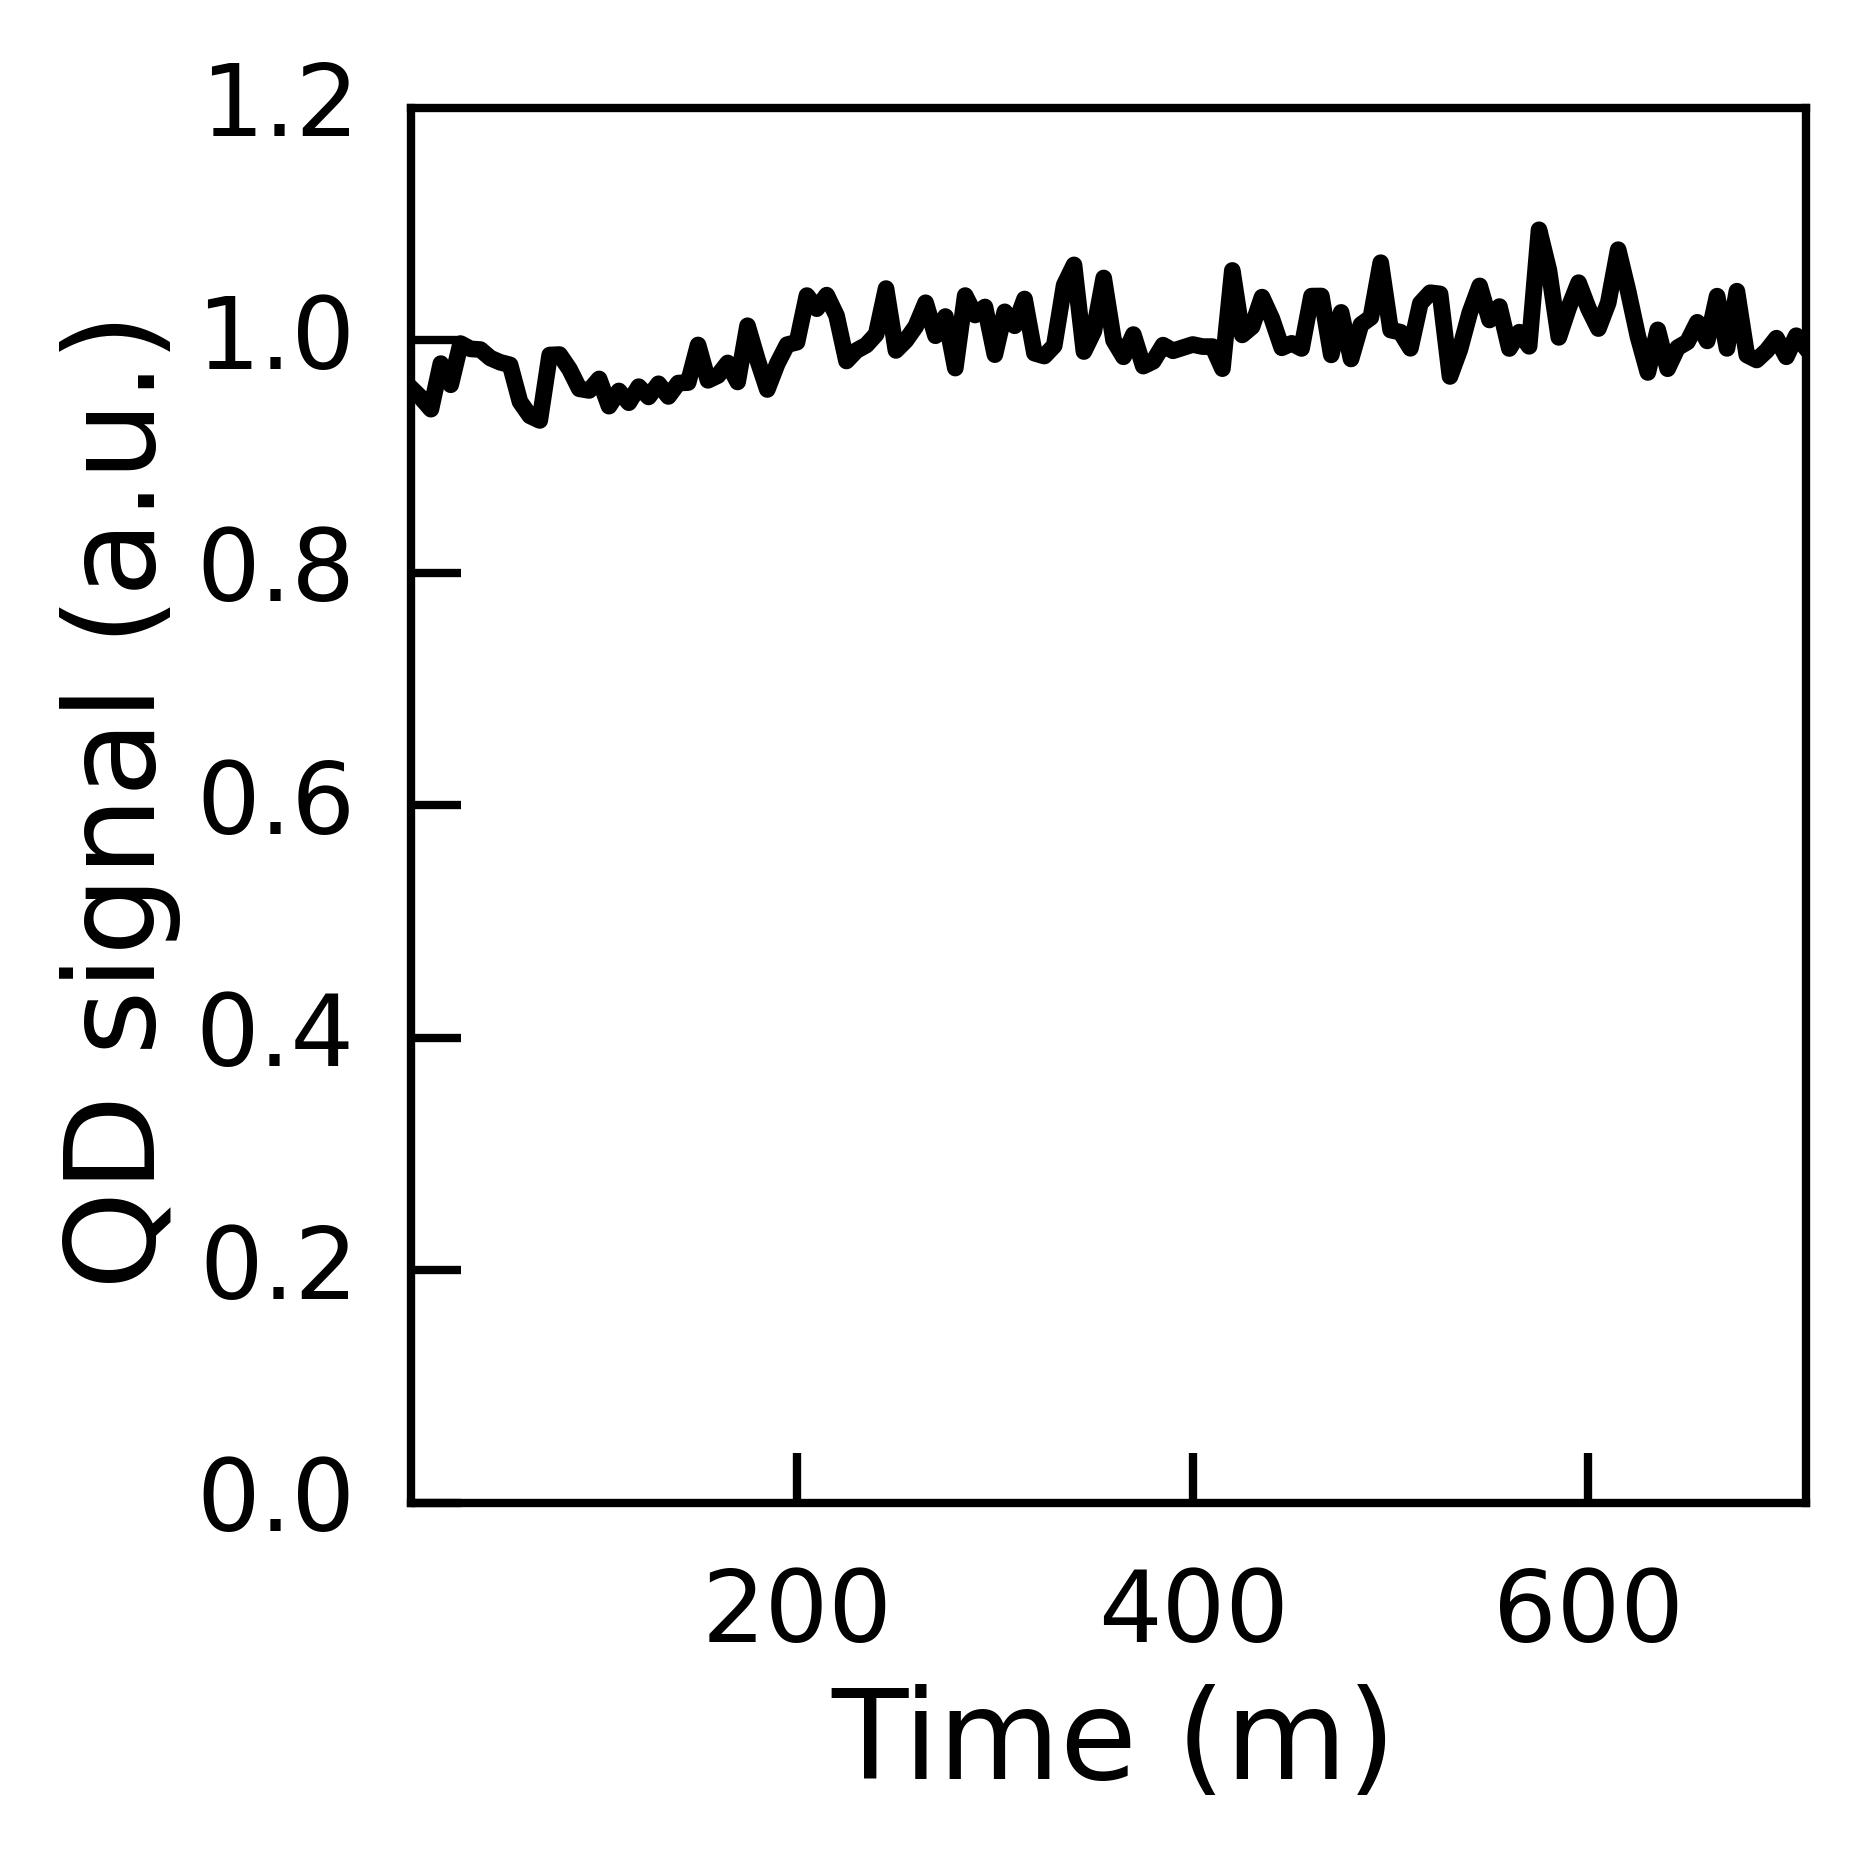
\includegraphics[width=0.45\textwidth]{images/stability.png} \caption{Counts
measured as a function of time over 12 hours.} \label{fig:stab} \end{center}
\end{figure}

To verify the single photon nature of the QD emission, a Hanbury Brown and Twiss
experiment was recorded using the on-chip MZ as a beamsplitter. The emission
from both arms was sent through two different transmission gratings for spectral
filtering and then sent to avalanche photodiodes. The signal in one arm was
delayed so as to measure negative correlation times. An absence of correlation
coincidences at time $\tau = 0$ implies single photon emission. The second order
correlation curves were taken under continuous wave ($\lambda$ = 810nm) and
pulsed ($\lambda$ = 850nm) excitation. The curves are shown in Figure
\ref{fig:g2s}. In the case of the pulsed curve (shown in Figure \ref{fig:g2s}
(a)) the signal to noise ratio due to dark counts, ($\sim \mathrm{100}$ vs $\sim
\mathrm{1500}$ QD counts), of the detectors was calculated and the resulting
dark count contribution was subtracted. A time window was also applied to the
data, since the lifetime of the QD was 670 $\pm$ 3ps, the vast majority (96\%)
of QD emission resides in a 4ns window. So only coincidences inside this window
were used for calculating the $g^{(2)}(0)$ value of 0.19.

\begin{figure}[h!] \begin{subfigure}{0.49\textwidth}
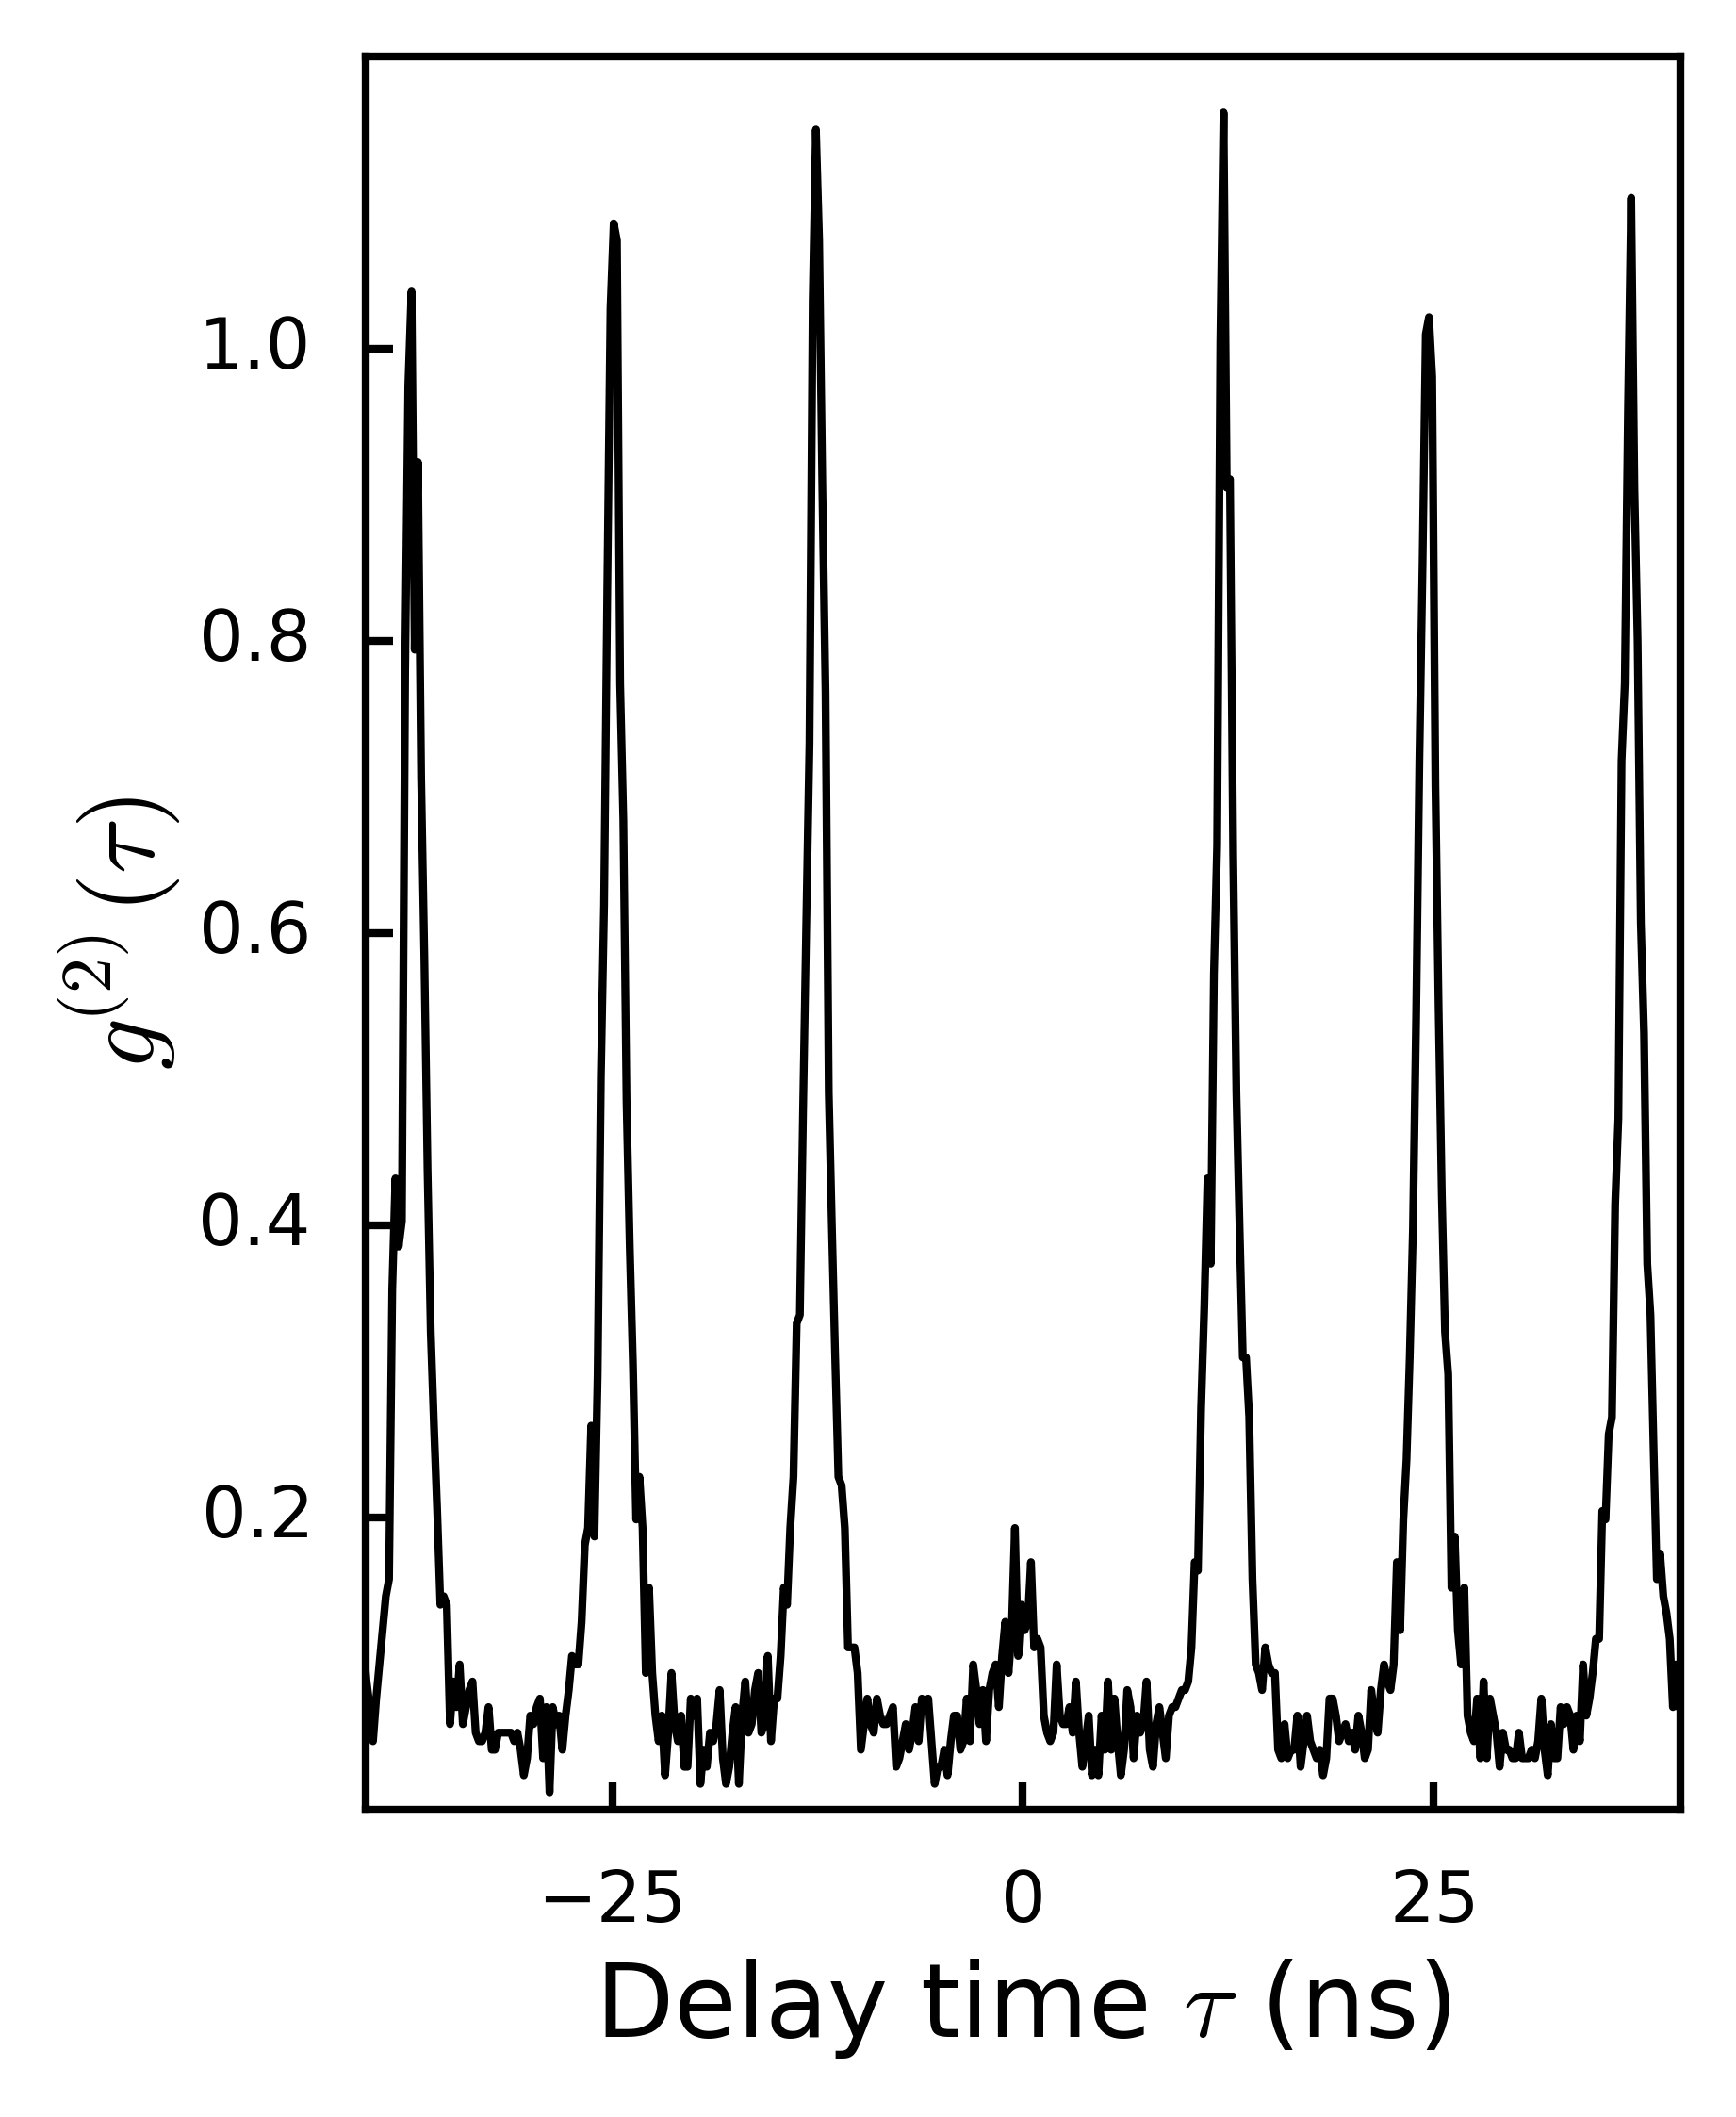
\includegraphics[width=1\textwidth]{images/g2_pulse.png} \label{fig:g2p}
\end{subfigure} \begin{subfigure}{0.49\textwidth}
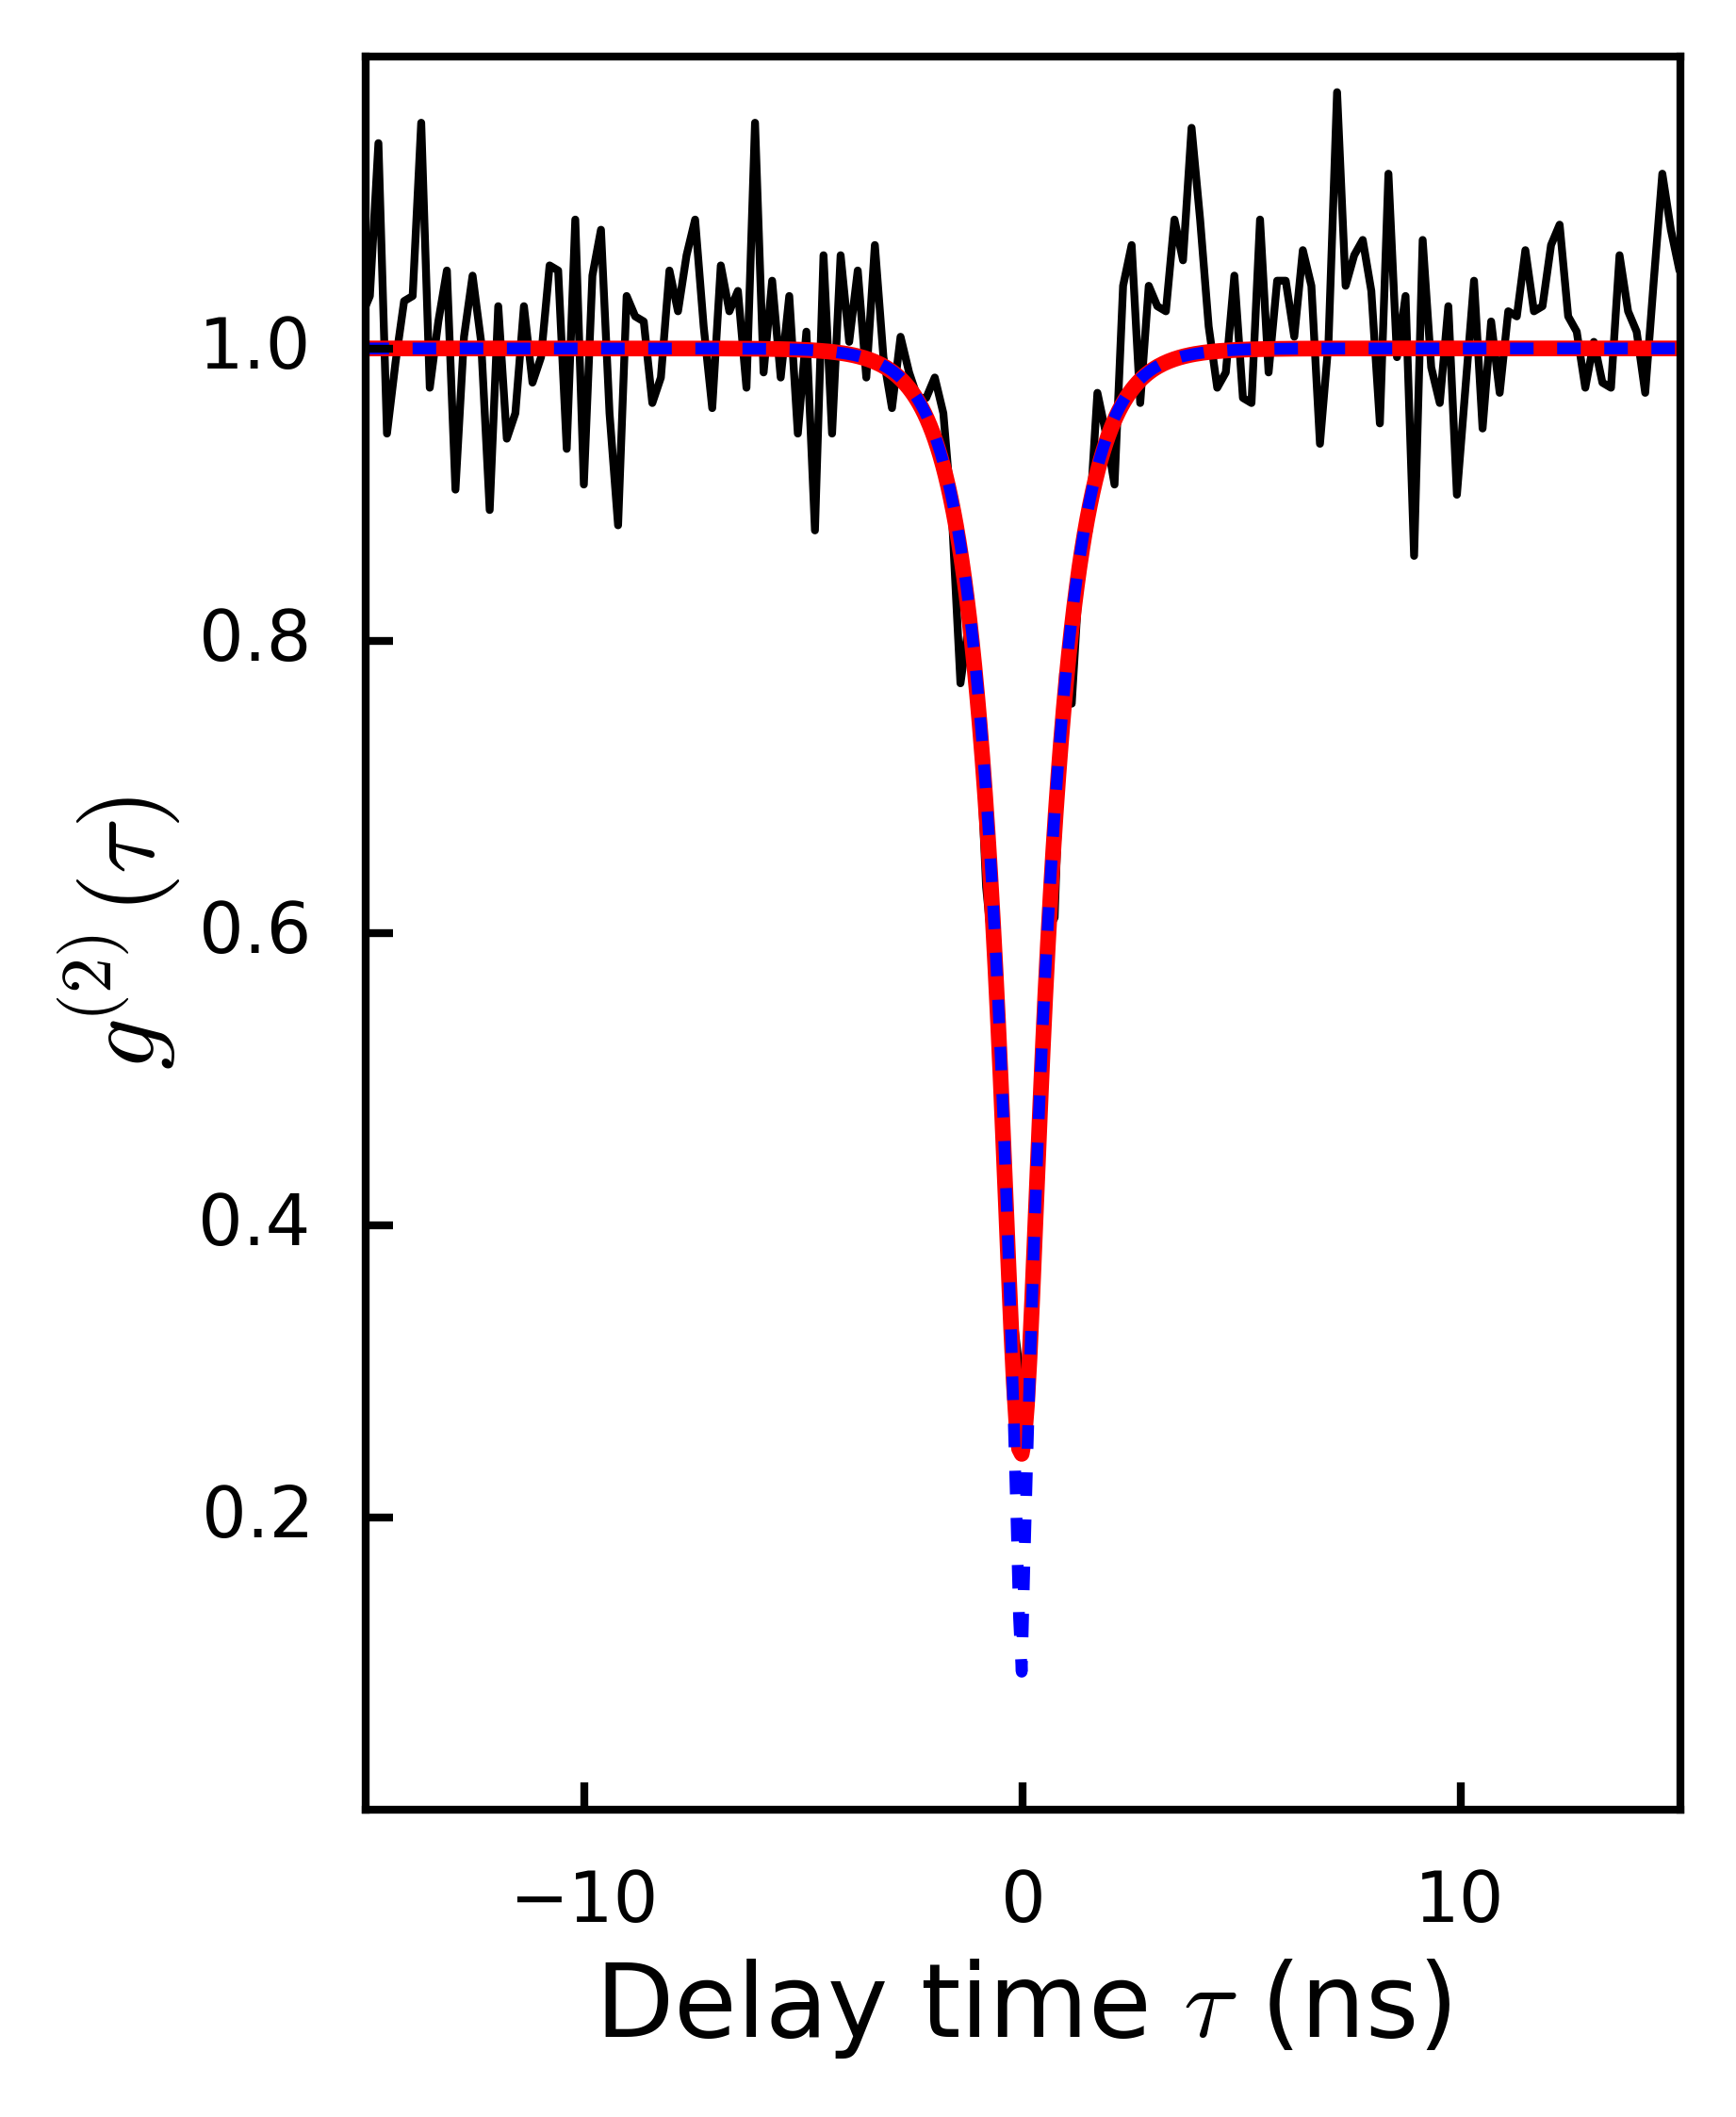
\includegraphics[width=1\textwidth]{images/g2_cw.png} \label{fig:g2cw}
\end{subfigure} \caption{(a) Second order correlation function under pulsed
excitation (b) Second order correlation function under continuous wave
excitation. The black line is the raw data, the red line is a fit taking the
system response funtion into account, and the dashed blue line is the fit
deconvoluted with the response function.} \label{fig:g2s} \end{figure}

In the CW case as seen in Figure \ref{fig:g2s} (b) the black line corresponds to
the data, the red solid line corresponds to a fit and the blue line to a
deconvoluted fit. The deconvolution was done to subtract the response function
of the detectors and timing system. The $g^{(2)}(0)$ was taken from the
deconvoluted to be 0.09.

\begin{figure}[h!] \centering
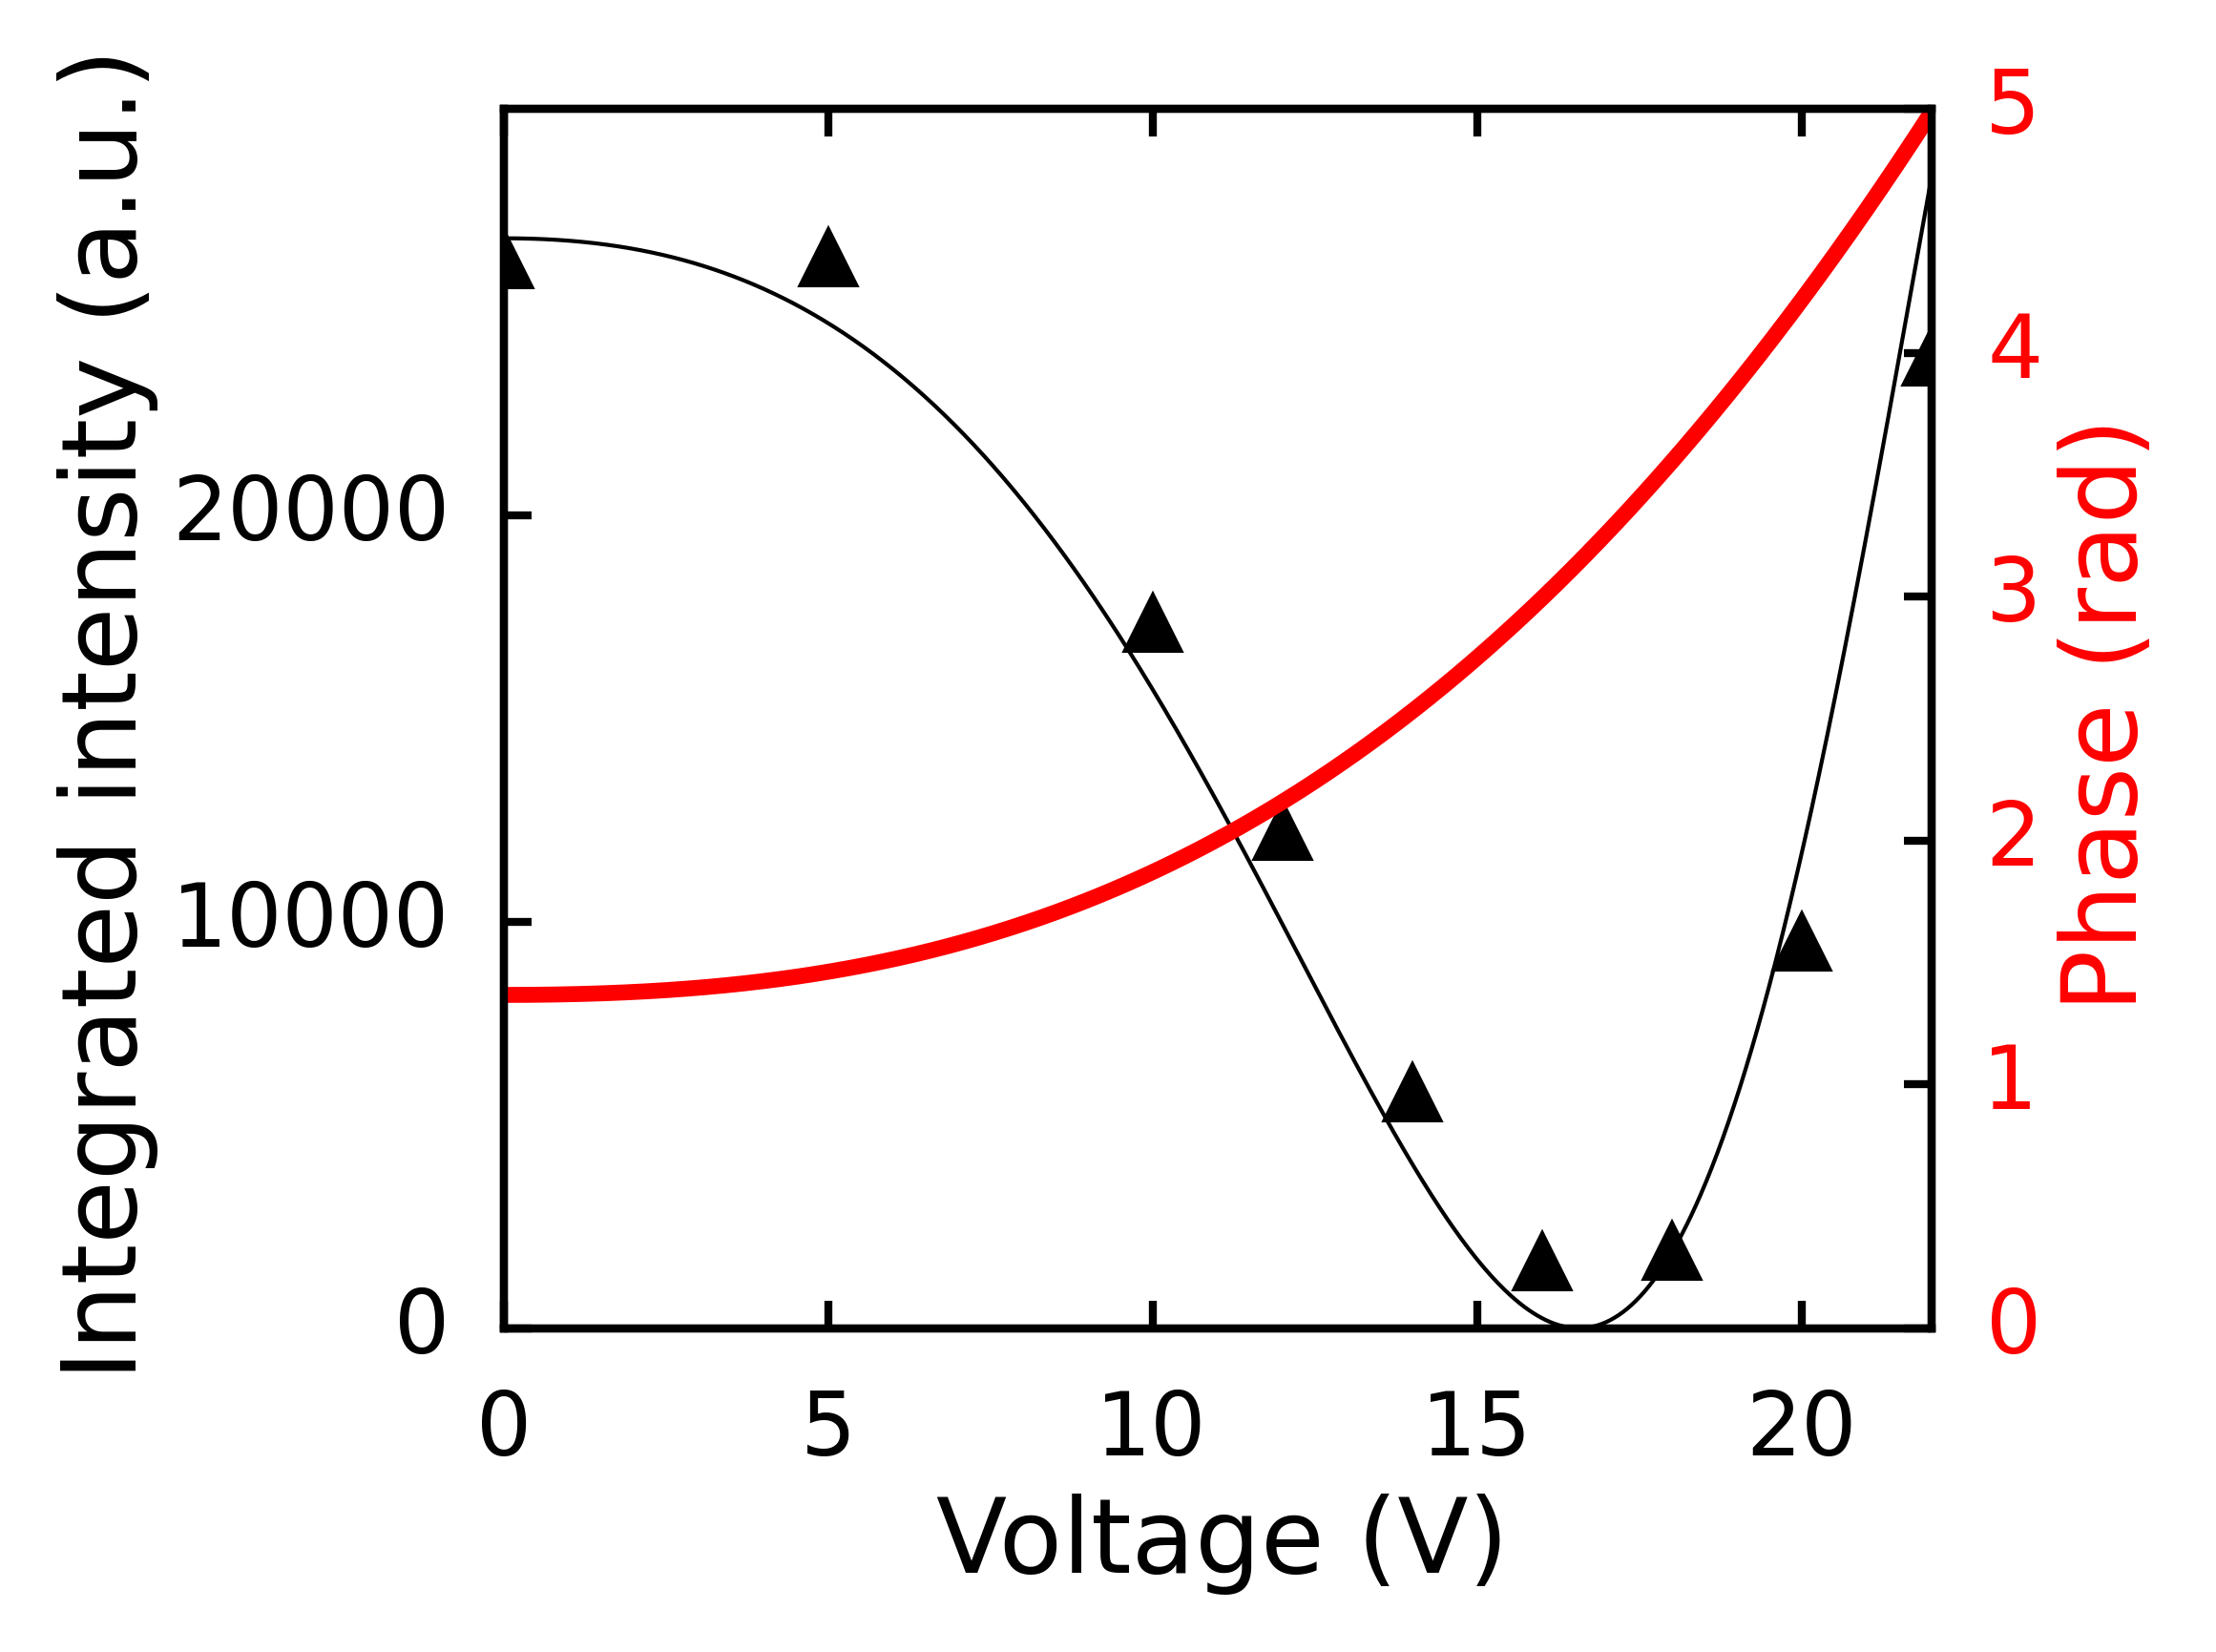
\includegraphics[width=0.6\textwidth]{images/dj_oneport.png} \caption{The
outputs a MZ arm is shown by the black triangles, the solid black line is a fit
to the data. The red line is the calculated phase as a function of voltage.}
\label{fig:modul} \end{figure}

The active modulation of the MZ was tested on the single photon source. A
voltage was applied to the heater on one arm of the MZ which induces local
heating of the arm and a change in the refractive index of the waveguide core.
This creates a relative phase between the light in each arm. The emission
coupling to each output arm of the MZ then varies as a function of the applied
voltage. This coupling, along with calculated phase, is shown in Figure
\ref{fig:modul}.

The model was based on calculating the expected power output of each port as a
function of coupling ratio and phase. The expected power is based on the matrix
model of a phase shift operation between two directional couplers
\cite{jones1941new}. The model of the phase the same as the one used in Section
\ref{sec:wg_devices}\cite{matthews2009manipulation}.

\subsubsection{Multiplexed source}

In conclusion a novel method for integrating a III-V quantum light source with
an SiON waveguide platform has been demonstrated. The single photon nature of
the source was verified using on-chip components and the active modulation of
the emission was demonstrated. This device shows potential for integration of
site controlled \cite{juska2013towards} QDs granting precise alignment of
multiple QDs with multiple waveguides allowing for scalable quantum
manipulation.
